% Generated by Sphinx.
\def\sphinxdocclass{report}
\documentclass[letterpaper,10pt,english]{sphinxmanual}
\usepackage[utf8]{inputenc}
\DeclareUnicodeCharacter{00A0}{\nobreakspace}
\usepackage{cmap}
\usepackage[T1]{fontenc}
\usepackage{babel}
\usepackage{times}
\usepackage[Bjarne]{fncychap}
\usepackage{longtable}
\usepackage{sphinx}
\usepackage{multirow}


\title{HAllA: Hierarchical All-against All Documentation}
\date{November 26, 2013}
\release{0.0.1}
\author{Yo Sup Moon, Curtis Huttenhower}
\newcommand{\sphinxlogo}{}
\renewcommand{\releasename}{Release}
\makeindex

\makeatletter
\def\PYG@reset{\let\PYG@it=\relax \let\PYG@bf=\relax%
    \let\PYG@ul=\relax \let\PYG@tc=\relax%
    \let\PYG@bc=\relax \let\PYG@ff=\relax}
\def\PYG@tok#1{\csname PYG@tok@#1\endcsname}
\def\PYG@toks#1+{\ifx\relax#1\empty\else%
    \PYG@tok{#1}\expandafter\PYG@toks\fi}
\def\PYG@do#1{\PYG@bc{\PYG@tc{\PYG@ul{%
    \PYG@it{\PYG@bf{\PYG@ff{#1}}}}}}}
\def\PYG#1#2{\PYG@reset\PYG@toks#1+\relax+\PYG@do{#2}}

\expandafter\def\csname PYG@tok@gd\endcsname{\def\PYG@tc##1{\textcolor[rgb]{0.63,0.00,0.00}{##1}}}
\expandafter\def\csname PYG@tok@gu\endcsname{\let\PYG@bf=\textbf\def\PYG@tc##1{\textcolor[rgb]{0.50,0.00,0.50}{##1}}}
\expandafter\def\csname PYG@tok@gt\endcsname{\def\PYG@tc##1{\textcolor[rgb]{0.00,0.27,0.87}{##1}}}
\expandafter\def\csname PYG@tok@gs\endcsname{\let\PYG@bf=\textbf}
\expandafter\def\csname PYG@tok@gr\endcsname{\def\PYG@tc##1{\textcolor[rgb]{1.00,0.00,0.00}{##1}}}
\expandafter\def\csname PYG@tok@cm\endcsname{\let\PYG@it=\textit\def\PYG@tc##1{\textcolor[rgb]{0.25,0.50,0.56}{##1}}}
\expandafter\def\csname PYG@tok@vg\endcsname{\def\PYG@tc##1{\textcolor[rgb]{0.73,0.38,0.84}{##1}}}
\expandafter\def\csname PYG@tok@m\endcsname{\def\PYG@tc##1{\textcolor[rgb]{0.13,0.50,0.31}{##1}}}
\expandafter\def\csname PYG@tok@mh\endcsname{\def\PYG@tc##1{\textcolor[rgb]{0.13,0.50,0.31}{##1}}}
\expandafter\def\csname PYG@tok@cs\endcsname{\def\PYG@tc##1{\textcolor[rgb]{0.25,0.50,0.56}{##1}}\def\PYG@bc##1{\setlength{\fboxsep}{0pt}\colorbox[rgb]{1.00,0.94,0.94}{\strut ##1}}}
\expandafter\def\csname PYG@tok@ge\endcsname{\let\PYG@it=\textit}
\expandafter\def\csname PYG@tok@vc\endcsname{\def\PYG@tc##1{\textcolor[rgb]{0.73,0.38,0.84}{##1}}}
\expandafter\def\csname PYG@tok@il\endcsname{\def\PYG@tc##1{\textcolor[rgb]{0.13,0.50,0.31}{##1}}}
\expandafter\def\csname PYG@tok@go\endcsname{\def\PYG@tc##1{\textcolor[rgb]{0.20,0.20,0.20}{##1}}}
\expandafter\def\csname PYG@tok@cp\endcsname{\def\PYG@tc##1{\textcolor[rgb]{0.00,0.44,0.13}{##1}}}
\expandafter\def\csname PYG@tok@gi\endcsname{\def\PYG@tc##1{\textcolor[rgb]{0.00,0.63,0.00}{##1}}}
\expandafter\def\csname PYG@tok@gh\endcsname{\let\PYG@bf=\textbf\def\PYG@tc##1{\textcolor[rgb]{0.00,0.00,0.50}{##1}}}
\expandafter\def\csname PYG@tok@ni\endcsname{\let\PYG@bf=\textbf\def\PYG@tc##1{\textcolor[rgb]{0.84,0.33,0.22}{##1}}}
\expandafter\def\csname PYG@tok@nl\endcsname{\let\PYG@bf=\textbf\def\PYG@tc##1{\textcolor[rgb]{0.00,0.13,0.44}{##1}}}
\expandafter\def\csname PYG@tok@nn\endcsname{\let\PYG@bf=\textbf\def\PYG@tc##1{\textcolor[rgb]{0.05,0.52,0.71}{##1}}}
\expandafter\def\csname PYG@tok@no\endcsname{\def\PYG@tc##1{\textcolor[rgb]{0.38,0.68,0.84}{##1}}}
\expandafter\def\csname PYG@tok@na\endcsname{\def\PYG@tc##1{\textcolor[rgb]{0.25,0.44,0.63}{##1}}}
\expandafter\def\csname PYG@tok@nb\endcsname{\def\PYG@tc##1{\textcolor[rgb]{0.00,0.44,0.13}{##1}}}
\expandafter\def\csname PYG@tok@nc\endcsname{\let\PYG@bf=\textbf\def\PYG@tc##1{\textcolor[rgb]{0.05,0.52,0.71}{##1}}}
\expandafter\def\csname PYG@tok@nd\endcsname{\let\PYG@bf=\textbf\def\PYG@tc##1{\textcolor[rgb]{0.33,0.33,0.33}{##1}}}
\expandafter\def\csname PYG@tok@ne\endcsname{\def\PYG@tc##1{\textcolor[rgb]{0.00,0.44,0.13}{##1}}}
\expandafter\def\csname PYG@tok@nf\endcsname{\def\PYG@tc##1{\textcolor[rgb]{0.02,0.16,0.49}{##1}}}
\expandafter\def\csname PYG@tok@si\endcsname{\let\PYG@it=\textit\def\PYG@tc##1{\textcolor[rgb]{0.44,0.63,0.82}{##1}}}
\expandafter\def\csname PYG@tok@s2\endcsname{\def\PYG@tc##1{\textcolor[rgb]{0.25,0.44,0.63}{##1}}}
\expandafter\def\csname PYG@tok@vi\endcsname{\def\PYG@tc##1{\textcolor[rgb]{0.73,0.38,0.84}{##1}}}
\expandafter\def\csname PYG@tok@nt\endcsname{\let\PYG@bf=\textbf\def\PYG@tc##1{\textcolor[rgb]{0.02,0.16,0.45}{##1}}}
\expandafter\def\csname PYG@tok@nv\endcsname{\def\PYG@tc##1{\textcolor[rgb]{0.73,0.38,0.84}{##1}}}
\expandafter\def\csname PYG@tok@s1\endcsname{\def\PYG@tc##1{\textcolor[rgb]{0.25,0.44,0.63}{##1}}}
\expandafter\def\csname PYG@tok@gp\endcsname{\let\PYG@bf=\textbf\def\PYG@tc##1{\textcolor[rgb]{0.78,0.36,0.04}{##1}}}
\expandafter\def\csname PYG@tok@sh\endcsname{\def\PYG@tc##1{\textcolor[rgb]{0.25,0.44,0.63}{##1}}}
\expandafter\def\csname PYG@tok@ow\endcsname{\let\PYG@bf=\textbf\def\PYG@tc##1{\textcolor[rgb]{0.00,0.44,0.13}{##1}}}
\expandafter\def\csname PYG@tok@sx\endcsname{\def\PYG@tc##1{\textcolor[rgb]{0.78,0.36,0.04}{##1}}}
\expandafter\def\csname PYG@tok@bp\endcsname{\def\PYG@tc##1{\textcolor[rgb]{0.00,0.44,0.13}{##1}}}
\expandafter\def\csname PYG@tok@c1\endcsname{\let\PYG@it=\textit\def\PYG@tc##1{\textcolor[rgb]{0.25,0.50,0.56}{##1}}}
\expandafter\def\csname PYG@tok@kc\endcsname{\let\PYG@bf=\textbf\def\PYG@tc##1{\textcolor[rgb]{0.00,0.44,0.13}{##1}}}
\expandafter\def\csname PYG@tok@c\endcsname{\let\PYG@it=\textit\def\PYG@tc##1{\textcolor[rgb]{0.25,0.50,0.56}{##1}}}
\expandafter\def\csname PYG@tok@mf\endcsname{\def\PYG@tc##1{\textcolor[rgb]{0.13,0.50,0.31}{##1}}}
\expandafter\def\csname PYG@tok@err\endcsname{\def\PYG@bc##1{\setlength{\fboxsep}{0pt}\fcolorbox[rgb]{1.00,0.00,0.00}{1,1,1}{\strut ##1}}}
\expandafter\def\csname PYG@tok@kd\endcsname{\let\PYG@bf=\textbf\def\PYG@tc##1{\textcolor[rgb]{0.00,0.44,0.13}{##1}}}
\expandafter\def\csname PYG@tok@ss\endcsname{\def\PYG@tc##1{\textcolor[rgb]{0.32,0.47,0.09}{##1}}}
\expandafter\def\csname PYG@tok@sr\endcsname{\def\PYG@tc##1{\textcolor[rgb]{0.14,0.33,0.53}{##1}}}
\expandafter\def\csname PYG@tok@mo\endcsname{\def\PYG@tc##1{\textcolor[rgb]{0.13,0.50,0.31}{##1}}}
\expandafter\def\csname PYG@tok@mi\endcsname{\def\PYG@tc##1{\textcolor[rgb]{0.13,0.50,0.31}{##1}}}
\expandafter\def\csname PYG@tok@kn\endcsname{\let\PYG@bf=\textbf\def\PYG@tc##1{\textcolor[rgb]{0.00,0.44,0.13}{##1}}}
\expandafter\def\csname PYG@tok@o\endcsname{\def\PYG@tc##1{\textcolor[rgb]{0.40,0.40,0.40}{##1}}}
\expandafter\def\csname PYG@tok@kr\endcsname{\let\PYG@bf=\textbf\def\PYG@tc##1{\textcolor[rgb]{0.00,0.44,0.13}{##1}}}
\expandafter\def\csname PYG@tok@s\endcsname{\def\PYG@tc##1{\textcolor[rgb]{0.25,0.44,0.63}{##1}}}
\expandafter\def\csname PYG@tok@kp\endcsname{\def\PYG@tc##1{\textcolor[rgb]{0.00,0.44,0.13}{##1}}}
\expandafter\def\csname PYG@tok@w\endcsname{\def\PYG@tc##1{\textcolor[rgb]{0.73,0.73,0.73}{##1}}}
\expandafter\def\csname PYG@tok@kt\endcsname{\def\PYG@tc##1{\textcolor[rgb]{0.56,0.13,0.00}{##1}}}
\expandafter\def\csname PYG@tok@sc\endcsname{\def\PYG@tc##1{\textcolor[rgb]{0.25,0.44,0.63}{##1}}}
\expandafter\def\csname PYG@tok@sb\endcsname{\def\PYG@tc##1{\textcolor[rgb]{0.25,0.44,0.63}{##1}}}
\expandafter\def\csname PYG@tok@k\endcsname{\let\PYG@bf=\textbf\def\PYG@tc##1{\textcolor[rgb]{0.00,0.44,0.13}{##1}}}
\expandafter\def\csname PYG@tok@se\endcsname{\let\PYG@bf=\textbf\def\PYG@tc##1{\textcolor[rgb]{0.25,0.44,0.63}{##1}}}
\expandafter\def\csname PYG@tok@sd\endcsname{\let\PYG@it=\textit\def\PYG@tc##1{\textcolor[rgb]{0.25,0.44,0.63}{##1}}}

\def\PYGZbs{\char`\\}
\def\PYGZus{\char`\_}
\def\PYGZob{\char`\{}
\def\PYGZcb{\char`\}}
\def\PYGZca{\char`\^}
\def\PYGZam{\char`\&}
\def\PYGZlt{\char`\<}
\def\PYGZgt{\char`\>}
\def\PYGZsh{\char`\#}
\def\PYGZpc{\char`\%}
\def\PYGZdl{\char`\$}
\def\PYGZhy{\char`\-}
\def\PYGZsq{\char`\'}
\def\PYGZdq{\char`\"}
\def\PYGZti{\char`\~}
% for compatibility with earlier versions
\def\PYGZat{@}
\def\PYGZlb{[}
\def\PYGZrb{]}
\makeatother

\begin{document}

\maketitle
\tableofcontents
\phantomsection\label{index::doc}



\chapter{Version 0.0.1}
\label{index:halla-hierarchical-all-against-all-association-testing}\label{index:version-0-0-1}\begin{description}
\item[{Authors}] \leavevmode
Yo Sup Moon, Curtis Huttenhower

\item[{Google Group}] \leavevmode
halla-users: \href{https://groups.google.com/forum/\#!forum/halla-users}{https://groups.google.com/forum/\#!forum/halla-users}

\item[{License}] \leavevmode
MIT License

\item[{URL}] \leavevmode
\href{http://huttenhower.sph.harvard.edu/halla}{http://huttenhower.sph.harvard.edu/halla}

\item[{Citation}] \leavevmode
Yo Sup Moon, Curtis Huttenhower, ``Retrieving Signal from Noise in Big Data: An Information-Theoretic Approach to Hierarchical Exploratory Data Analysis'' (In Preparation)

\end{description}


\section{Chapter 0 Getting Started}
\label{index:chapter-0-getting-started}

\subsection{Operating System}
\label{index:operating-system}\begin{itemize}
\item {} \begin{description}
\item[{Supported}] \leavevmode\begin{itemize}
\item {} 
Ubuntu Linux (\textgreater{}= 12.04)

\item {} 
Mac OS X (\textgreater{}= 10.7)

\end{itemize}

\end{description}

\item {} \begin{description}
\item[{Unsupported}] \leavevmode\begin{itemize}
\item {} 
Windows (\textgreater{}= XP)

\end{itemize}

\end{description}

\end{itemize}


\subsection{Dependencies}
\label{index:dependencies}\begin{itemize}
\item {} \begin{description}
\item[{Required}] \leavevmode\begin{itemize}
\item {} 
Python (\textgreater{}= 2.7)

\item {} 
Numpy (\textgreater{}= 1.7.1)

\item {} 
Scipy (\textgreater{}= 0.12)

\item {} 
Scikit-learn (\textgreater{}=0.13)

\item {} 
rpy (\textgreater{}=2.0)

\item {} 
sampledoc-master

\end{itemize}

\end{description}

\item {} \begin{description}
\item[{Recommended Tools for documentation}] \leavevmode\begin{itemize}
\item {} 
Docutils

\item {} 
itex2MML

\end{itemize}

\end{description}

\end{itemize}


\subsection{Getting HAllA}
\label{index:getting-halla}
HAllA can be downloaded from its bitbucket repository: \href{http://bitbucket.org/chuttenh/halla}{http://bitbucket.org/chuttenh/halla}.


\section{Chapter 1 Basics}
\label{index:chapter-1-basics}

\subsection{Introduction}
\label{index:introduction}
HAllA: is a programmatic tool for performing multiple association testing between two or more heterogeneous datasets, each containing a mixture of discrete, binary, or continuous data. HAllA is a robust and efficient alternative to traditional all-against-all association testing of variables. Its robustness relies on the usage of mutual information-based measures to calculate the degree to which two variables are related. Mutual-information is well-suited to serve as an all-purpose measure since it is well-behaved even when comparing two variables of different data types. Its efficiency relies on a hierarchical clustering scheme to reduce the number of tests necessary to discover interesting associations in datasets that contain potentially millions of genotypic and phenotypic data. In a traditional all-against-all association-testing scheme, the number of pairwise tests scale quadratically with the number of features in the data (O(N\textasciicircum{}2)). The sheer number of association tests dramatically reduces the power of standard hypothesis tests to discover relationships among variables. We introduce a hierarchical hypothesis-testing scheme to perform tiered testing on clusters of data to reduce computational time for comparisons. Hierarchical false discovery rate correction is implemented to curb discoveries of associations due to noise in the data.


\subsection{Input}
\label{index:input}
HAlLA by default takes a tab-delimited text file as an input, where each row describes feature (data/metadata) and each column represents an instance. In other words, input \emph{X} is a \emph{D x N} matrix where \emph{D} is the number of dimensions in each instance of the data and \emph{N} is the number of instances (samples). The ``edges'' of the matrix should contain labels of the data, if desired. The following is an example input

\begin{Verbatim}[commandchars=\\\{\}]
+-------+---------+---------+--------+
\textbar{}       \textbar{} Sample1 \textbar{} Sample2 \textbar{} Sample3\textbar{}
+-------+---------+---------+--------+
\textbar{} Data1 \textbar{} 0       \textbar{} 1       \textbar{} 2      \textbar{}
+-------+---------+---------+--------+
\textbar{} Data2 \textbar{} 1.5     \textbar{} 100.2   \textbar{} -30.7  \textbar{}
+-------+---------+---------+--------+
\end{Verbatim}


\subsection{Output}
\label{index:output}
HAllA by default prints a tab-delimited text file as output

\begin{Verbatim}[commandchars=\\\{\}]
+------+------+-------+------+------+
\textbar{} One  \textbar{} Two  \textbar{} MID   \textbar{} Pperm\textbar{} Pboot\textbar{}
+------+------+-------+------+------+
\textbar{} Data1\textbar{} Data2\textbar{} 0.64  \textbar{} 0.02 \textbar{} 0.008\textbar{}
+------+------+-------+------+------+
\end{Verbatim}

\emph{MID} stands for ``mutual information distance'', which is an information-theoretic measure of association between two random variables. \emph{Pperm} and \emph{Pboot} corresponds to the p-values of the permutation and bootstrap tests used to assess the statistical significance of the mutual information distance (i.e. lower p-values signify that the association between two variables
is not likely to be caused by the noise in the data).


\subsection{Advanced}
\label{index:advanced}
The following is a list of all available arguments that can be passed into halla:

\begin{Verbatim}[commandchars=\\\{\}]
usage: halla.py [-h] [-o output.txt] [-p p\_value] [-P p\_mi] [-b bootstraps] [-v verbosity] [input.txt]

Hierarchical All-against-All significance association testing.

positional arguments:
  input.txt      Tab-delimited text input file, one row per feature, one
                 column per measurement

optional arguments:
  -h, --help     show this help message and exit
  -o output.txt  Optional output file for association significance tests
  -p p\_value     P-value for overall significance tests
  -P p\_mi        P-value for permutation equivalence of MI clusters
  -b bootstraps  Number of bootstraps for significance testing
  -v verbosity   Debug logging level; increase for greater verbosity
\end{Verbatim}


\subsection{Mini-tutorial}
\label{index:mini-tutorial}
Suppose you have a tab-delimited file containing the dataset you wish to run halla on. We will call this file \emph{in.txt}. We will call the output file \emph{out.txt}. In the root directory of halla, one can type:

\begin{Verbatim}[commandchars=\\\{\}]
\$ python halla.py in.txt \textgreater{} out.txt
\end{Verbatim}

To obtain the output in \emph{out.txt}.


\section{Frequently Asked Questions}
\label{index:frequently-asked-questions}
NB: Direct all questions to the halla-users google group.


\section{Functions}
\label{index:module-halla}\label{index:functions}\index{halla (module)}

\subsection{HAllA: Hiearchical All-against All}
\label{index:halla-hiearchical-all-against-all}\begin{description}
\item[{Description}] \leavevmode
An object-oriented halla implementation 
Aim to be as self-contained as possible

\end{description}

Global namespace conventions:
\begin{itemize}
\item {} 
\emph{m()} \textless{}- map for arrays

\item {} 
\emph{r()} \textless{}- reduce for arrays

\item {} 
\emph{rd()} \textless{}- generic reduce-dimension method

\end{itemize}
\index{multinomial() (in module halla)}

\begin{fulllineitems}
\phantomsection\label{index:halla.multinomial}\pysiglinewithargsret{\code{halla.}\bfcode{multinomial}}{\emph{n}, \emph{pvals}, \emph{size=None}}{}
Draw samples from a multinomial distribution.

The multinomial distribution is a multivariate generalisation of the
binomial distribution.  Take an experiment with one of \code{p}
possible outcomes.  An example of such an experiment is throwing a dice,
where the outcome can be 1 through 6.  Each sample drawn from the
distribution represents \emph{n} such experiments.  Its values,
\code{X\_i = {[}X\_0, X\_1, ..., X\_p{]}}, represent the number of times the outcome
was \code{i}.
\begin{description}
\item[{n}] \leavevmode{[}int{]}
Number of experiments.

\item[{pvals}] \leavevmode{[}sequence of floats, length p{]}
Probabilities of each of the \code{p} different outcomes.  These
should sum to 1 (however, the last element is always assumed to
account for the remaining probability, as long as
\code{sum(pvals{[}:-1{]}) \textless{}= 1)}.

\item[{size}] \leavevmode{[}tuple of ints{]}
Given a \emph{size} of \code{(M, N, K)}, then \code{M*N*K} samples are drawn,
and the output shape becomes \code{(M, N, K, p)}, since each sample
has shape \code{(p,)}.

\end{description}

Throw a dice 20 times:

\begin{Verbatim}[commandchars=\\\{\}]
\PYG{g+gp}{\PYGZgt{}\PYGZgt{}\PYGZgt{} }\PYG{n}{np}\PYG{o}{.}\PYG{n}{random}\PYG{o}{.}\PYG{n}{multinomial}\PYG{p}{(}\PYG{l+m+mi}{20}\PYG{p}{,} \PYG{p}{[}\PYG{l+m+mi}{1}\PYG{o}{/}\PYG{l+m+mf}{6.}\PYG{p}{]}\PYG{o}{*}\PYG{l+m+mi}{6}\PYG{p}{,} \PYG{n}{size}\PYG{o}{=}\PYG{l+m+mi}{1}\PYG{p}{)}
\PYG{g+go}{array([[4, 1, 7, 5, 2, 1]])}
\end{Verbatim}

It landed 4 times on 1, once on 2, etc.

Now, throw the dice 20 times, and 20 times again:

\begin{Verbatim}[commandchars=\\\{\}]
\PYG{g+gp}{\PYGZgt{}\PYGZgt{}\PYGZgt{} }\PYG{n}{np}\PYG{o}{.}\PYG{n}{random}\PYG{o}{.}\PYG{n}{multinomial}\PYG{p}{(}\PYG{l+m+mi}{20}\PYG{p}{,} \PYG{p}{[}\PYG{l+m+mi}{1}\PYG{o}{/}\PYG{l+m+mf}{6.}\PYG{p}{]}\PYG{o}{*}\PYG{l+m+mi}{6}\PYG{p}{,} \PYG{n}{size}\PYG{o}{=}\PYG{l+m+mi}{2}\PYG{p}{)}
\PYG{g+go}{array([[3, 4, 3, 3, 4, 3],}
\PYG{g+go}{       [2, 4, 3, 4, 0, 7]])}
\end{Verbatim}

For the first run, we threw 3 times 1, 4 times 2, etc.  For the second,
we threw 2 times 1, 4 times 2, etc.

A loaded dice is more likely to land on number 6:

\begin{Verbatim}[commandchars=\\\{\}]
\PYG{g+gp}{\PYGZgt{}\PYGZgt{}\PYGZgt{} }\PYG{n}{np}\PYG{o}{.}\PYG{n}{random}\PYG{o}{.}\PYG{n}{multinomial}\PYG{p}{(}\PYG{l+m+mi}{100}\PYG{p}{,} \PYG{p}{[}\PYG{l+m+mi}{1}\PYG{o}{/}\PYG{l+m+mf}{7.}\PYG{p}{]}\PYG{o}{*}\PYG{l+m+mi}{5}\PYG{p}{)}
\PYG{g+go}{array([13, 16, 13, 16, 42])}
\end{Verbatim}

\end{fulllineitems}

\index{normal() (in module halla)}

\begin{fulllineitems}
\phantomsection\label{index:halla.normal}\pysiglinewithargsret{\code{halla.}\bfcode{normal}}{\emph{loc=0.0}, \emph{scale=1.0}, \emph{size=None}}{}
Draw random samples from a normal (Gaussian) distribution.

The probability density function of the normal distribution, first
derived by De Moivre and 200 years later by both Gauss and Laplace
independently {\color{red}\bfseries{}{[}2{]}\_}, is often called the bell curve because of
its characteristic shape (see the example below).

The normal distributions occurs often in nature.  For example, it
describes the commonly occurring distribution of samples influenced
by a large number of tiny, random disturbances, each with its own
unique distribution {\color{red}\bfseries{}{[}2{]}\_}.
\begin{description}
\item[{loc}] \leavevmode{[}float{]}
Mean (``centre'') of the distribution.

\item[{scale}] \leavevmode{[}float{]}
Standard deviation (spread or ``width'') of the distribution.

\item[{size}] \leavevmode{[}tuple of ints{]}
Output shape.  If the given shape is, e.g., \code{(m, n, k)}, then
\code{m * n * k} samples are drawn.

\end{description}
\begin{description}
\item[{scipy.stats.distributions.norm}] \leavevmode{[}probability density function,{]}
distribution or cumulative density function, etc.

\end{description}

The probability density for the Gaussian distribution is
\begin{equation}p(x) = \frac{1}{\sqrt{ 2 \pi \sigma^2 }}e^{ - \frac{ (x - \mu)^2 } {2 \sigma^2} },\end{equation}
where $\mu$ is the mean and $\sigma$ the standard deviation.
The square of the standard deviation, $\sigma^2$, is called the
variance.

The function has its peak at the mean, and its ``spread'' increases with
the standard deviation (the function reaches 0.607 times its maximum at
$x + \sigma$ and $x - \sigma$ {\color{red}\bfseries{}{[}2{]}\_}).  This implies that
\emph{numpy.random.normal} is more likely to return samples lying close to the
mean, rather than those far away.

Draw samples from the distribution:

\begin{Verbatim}[commandchars=\\\{\}]
\PYG{g+gp}{\PYGZgt{}\PYGZgt{}\PYGZgt{} }\PYG{n}{mu}\PYG{p}{,} \PYG{n}{sigma} \PYG{o}{=} \PYG{l+m+mi}{0}\PYG{p}{,} \PYG{l+m+mf}{0.1} \PYG{c}{\PYGZsh{} mean and standard deviation}
\PYG{g+gp}{\PYGZgt{}\PYGZgt{}\PYGZgt{} }\PYG{n}{s} \PYG{o}{=} \PYG{n}{np}\PYG{o}{.}\PYG{n}{random}\PYG{o}{.}\PYG{n}{normal}\PYG{p}{(}\PYG{n}{mu}\PYG{p}{,} \PYG{n}{sigma}\PYG{p}{,} \PYG{l+m+mi}{1000}\PYG{p}{)}
\end{Verbatim}

Verify the mean and the variance:

\begin{Verbatim}[commandchars=\\\{\}]
\PYG{g+gp}{\PYGZgt{}\PYGZgt{}\PYGZgt{} }\PYG{n+nb}{abs}\PYG{p}{(}\PYG{n}{mu} \PYG{o}{\PYGZhy{}} \PYG{n}{np}\PYG{o}{.}\PYG{n}{mean}\PYG{p}{(}\PYG{n}{s}\PYG{p}{)}\PYG{p}{)} \PYG{o}{\PYGZlt{}} \PYG{l+m+mf}{0.01}
\PYG{g+go}{True}
\end{Verbatim}

\begin{Verbatim}[commandchars=\\\{\}]
\PYG{g+gp}{\PYGZgt{}\PYGZgt{}\PYGZgt{} }\PYG{n+nb}{abs}\PYG{p}{(}\PYG{n}{sigma} \PYG{o}{\PYGZhy{}} \PYG{n}{np}\PYG{o}{.}\PYG{n}{std}\PYG{p}{(}\PYG{n}{s}\PYG{p}{,} \PYG{n}{ddof}\PYG{o}{=}\PYG{l+m+mi}{1}\PYG{p}{)}\PYG{p}{)} \PYG{o}{\PYGZlt{}} \PYG{l+m+mf}{0.01}
\PYG{g+go}{True}
\end{Verbatim}

Display the histogram of the samples, along with
the probability density function:

\begin{Verbatim}[commandchars=\\\{\}]
\PYG{g+gp}{\PYGZgt{}\PYGZgt{}\PYGZgt{} }\PYG{k+kn}{import} \PYG{n+nn}{matplotlib.pyplot} \PYG{k+kn}{as} \PYG{n+nn}{plt}
\PYG{g+gp}{\PYGZgt{}\PYGZgt{}\PYGZgt{} }\PYG{n}{count}\PYG{p}{,} \PYG{n}{bins}\PYG{p}{,} \PYG{n}{ignored} \PYG{o}{=} \PYG{n}{plt}\PYG{o}{.}\PYG{n}{hist}\PYG{p}{(}\PYG{n}{s}\PYG{p}{,} \PYG{l+m+mi}{30}\PYG{p}{,} \PYG{n}{normed}\PYG{o}{=}\PYG{n+nb+bp}{True}\PYG{p}{)}
\PYG{g+gp}{\PYGZgt{}\PYGZgt{}\PYGZgt{} }\PYG{n}{plt}\PYG{o}{.}\PYG{n}{plot}\PYG{p}{(}\PYG{n}{bins}\PYG{p}{,} \PYG{l+m+mi}{1}\PYG{o}{/}\PYG{p}{(}\PYG{n}{sigma} \PYG{o}{*} \PYG{n}{np}\PYG{o}{.}\PYG{n}{sqrt}\PYG{p}{(}\PYG{l+m+mi}{2} \PYG{o}{*} \PYG{n}{np}\PYG{o}{.}\PYG{n}{pi}\PYG{p}{)}\PYG{p}{)} \PYG{o}{*}
\PYG{g+gp}{... }               \PYG{n}{np}\PYG{o}{.}\PYG{n}{exp}\PYG{p}{(} \PYG{o}{\PYGZhy{}} \PYG{p}{(}\PYG{n}{bins} \PYG{o}{\PYGZhy{}} \PYG{n}{mu}\PYG{p}{)}\PYG{o}{*}\PYG{o}{*}\PYG{l+m+mi}{2} \PYG{o}{/} \PYG{p}{(}\PYG{l+m+mi}{2} \PYG{o}{*} \PYG{n}{sigma}\PYG{o}{*}\PYG{o}{*}\PYG{l+m+mi}{2}\PYG{p}{)} \PYG{p}{)}\PYG{p}{,}
\PYG{g+gp}{... }         \PYG{n}{linewidth}\PYG{o}{=}\PYG{l+m+mi}{2}\PYG{p}{,} \PYG{n}{color}\PYG{o}{=}\PYG{l+s}{\PYGZsq{}}\PYG{l+s}{r}\PYG{l+s}{\PYGZsq{}}\PYG{p}{)}
\PYG{g+gp}{\PYGZgt{}\PYGZgt{}\PYGZgt{} }\PYG{n}{plt}\PYG{o}{.}\PYG{n}{show}\PYG{p}{(}\PYG{p}{)}
\end{Verbatim}

\end{fulllineitems}

\phantomsection\label{index:module-halla.stats}\index{halla.stats (module)}
unified statistics module
\index{IBP\_cut() (in module halla.stats)}

\begin{fulllineitems}
\phantomsection\label{index:halla.stats.IBP_cut}\pysiglinewithargsret{\code{halla.stats.}\bfcode{IBP\_cut}}{\emph{cake\_length}}{}
random cut generated by Indian Buffet Process prior

\end{fulllineitems}

\index{PY\_cut() (in module halla.stats)}

\begin{fulllineitems}
\phantomsection\label{index:halla.stats.PY_cut}\pysiglinewithargsret{\code{halla.stats.}\bfcode{PY\_cut}}{\emph{cake\_length}}{}
random cut generated by pitman-yor process prior

\end{fulllineitems}

\index{bh() (in module halla.stats)}

\begin{fulllineitems}
\phantomsection\label{index:halla.stats.bh}\pysiglinewithargsret{\code{halla.stats.}\bfcode{bh}}{\emph{afPVAL}, \emph{fQ=1.0}}{}
Implement the benjamini-hochberg hierarchical hypothesis testing criterion 
In practice, used for implementing Yekutieli criterion \emph{per layer}.

When BH is performed per layer, FDR is approximately
\begin{equation}FDR = q \cdot \delta^{*} \cdot(m_0 + m_1)/(m_0+1)\end{equation}
where $m_0$ is the observed number of discoveries and $m_1$ is the observed number of families tested.

Universal bound: the full tree FDR is $< q \cdot \delta^{*} \cdot 2$
\begin{description}
\item[{\emph{afPVAL}}] \leavevmode
list of p-values

\item[{\emph{abOUT}}] \leavevmode
boolean vector corresponding to which hypothesis test rejected, corresponding to p-value

\end{description}

\end{fulllineitems}

\index{binomial() (in module halla.stats)}

\begin{fulllineitems}
\phantomsection\label{index:halla.stats.binomial}\pysiglinewithargsret{\code{halla.stats.}\bfcode{binomial}}{\emph{n}, \emph{p}, \emph{size=None}}{}
Draw samples from a binomial distribution.

Samples are drawn from a Binomial distribution with specified
parameters, n trials and p probability of success where
n an integer \textgreater{} 0 and p is in the interval {[}0,1{]}. (n may be
input as a float, but it is truncated to an integer in use)
\begin{description}
\item[{n}] \leavevmode{[}float (but truncated to an integer){]}
parameter, \textgreater{} 0.

\item[{p}] \leavevmode{[}float{]}
parameter, \textgreater{}= 0 and \textless{}=1.

\item[{size}] \leavevmode{[}\{tuple, int\}{]}
Output shape.  If the given shape is, e.g., \code{(m, n, k)}, then
\code{m * n * k} samples are drawn.

\end{description}
\begin{description}
\item[{samples}] \leavevmode{[}\{ndarray, scalar\}{]}
where the values are all integers in  {[}0, n{]}.

\end{description}
\begin{description}
\item[{scipy.stats.distributions.binom}] \leavevmode{[}probability density function,{]}
distribution or cumulative density function, etc.

\end{description}

The probability density for the Binomial distribution is
\begin{equation}P(N) = \binom{n}{N}p^N(1-p)^{n-N},\end{equation}
where $n$ is the number of trials, $p$ is the probability
of success, and $N$ is the number of successes.

When estimating the standard error of a proportion in a population by
using a random sample, the normal distribution works well unless the
product p*n \textless{}=5, where p = population proportion estimate, and n =
number of samples, in which case the binomial distribution is used
instead. For example, a sample of 15 people shows 4 who are left
handed, and 11 who are right handed. Then p = 4/15 = 27\%. 0.27*15 = 4,
so the binomial distribution should be used in this case.

Draw samples from the distribution:

\begin{Verbatim}[commandchars=\\\{\}]
\PYG{g+gp}{\PYGZgt{}\PYGZgt{}\PYGZgt{} }\PYG{n}{n}\PYG{p}{,} \PYG{n}{p} \PYG{o}{=} \PYG{l+m+mi}{10}\PYG{p}{,} \PYG{o}{.}\PYG{l+m+mi}{5} \PYG{c}{\PYGZsh{} number of trials, probability of each trial}
\PYG{g+gp}{\PYGZgt{}\PYGZgt{}\PYGZgt{} }\PYG{n}{s} \PYG{o}{=} \PYG{n}{np}\PYG{o}{.}\PYG{n}{random}\PYG{o}{.}\PYG{n}{binomial}\PYG{p}{(}\PYG{n}{n}\PYG{p}{,} \PYG{n}{p}\PYG{p}{,} \PYG{l+m+mi}{1000}\PYG{p}{)}
\PYG{g+go}{\PYGZsh{} result of flipping a coin 10 times, tested 1000 times.}
\end{Verbatim}

A real world example. A company drills 9 wild-cat oil exploration
wells, each with an estimated probability of success of 0.1. All nine
wells fail. What is the probability of that happening?

Let's do 20,000 trials of the model, and count the number that
generate zero positive results.

\begin{Verbatim}[commandchars=\\\{\}]
\PYG{g+gp}{\PYGZgt{}\PYGZgt{}\PYGZgt{} }\PYG{n+nb}{sum}\PYG{p}{(}\PYG{n}{np}\PYG{o}{.}\PYG{n}{random}\PYG{o}{.}\PYG{n}{binomial}\PYG{p}{(}\PYG{l+m+mi}{9}\PYG{p}{,}\PYG{l+m+mf}{0.1}\PYG{p}{,}\PYG{l+m+mi}{20000}\PYG{p}{)}\PYG{o}{==}\PYG{l+m+mi}{0}\PYG{p}{)}\PYG{o}{/}\PYG{l+m+mf}{20000.}
\PYG{g+go}{answer = 0.38885, or 38\PYGZpc{}.}
\end{Verbatim}

\end{fulllineitems}

\index{cumulative\_log\_cut() (in module halla.stats)}

\begin{fulllineitems}
\phantomsection\label{index:halla.stats.cumulative_log_cut}\pysiglinewithargsret{\code{halla.stats.}\bfcode{cumulative\_log\_cut}}{\emph{cake\_length}, \emph{iBase=2}}{}
Input: cake\_length \textless{}- length of array, iBase \textless{}- base of logarithm

Output: array of indices corresponding to the slice

Note: Probably don't want size-1 cake slices, but for proof-of-concept, this should be okay. 
Avoid the ``all'' case

\end{fulllineitems}

\index{discretize() (in module halla.stats)}

\begin{fulllineitems}
\phantomsection\label{index:halla.stats.discretize}\pysiglinewithargsret{\code{halla.stats.}\bfcode{discretize}}{\emph{pArray}, \emph{iN=None}, \emph{method=None}, \emph{aiSkip=}\optional{}}{}~
\begin{Verbatim}[commandchars=\\\{\}]
\PYG{g+gp}{\PYGZgt{}\PYGZgt{}\PYGZgt{} }\PYG{n}{discretize}\PYG{p}{(} \PYG{p}{[}\PYG{l+m+mf}{0.1}\PYG{p}{,} \PYG{l+m+mf}{0.2}\PYG{p}{,} \PYG{l+m+mf}{0.3}\PYG{p}{,} \PYG{l+m+mf}{0.4}\PYG{p}{]} \PYG{p}{)}
\PYG{g+go}{[0, 0, 1, 1]}
\end{Verbatim}

\begin{Verbatim}[commandchars=\\\{\}]
\PYG{g+gp}{\PYGZgt{}\PYGZgt{}\PYGZgt{} }\PYG{n}{discretize}\PYG{p}{(} \PYG{p}{[}\PYG{l+m+mf}{0.01}\PYG{p}{,} \PYG{l+m+mf}{0.04}\PYG{p}{,} \PYG{l+m+mf}{0.09}\PYG{p}{,} \PYG{l+m+mf}{0.16}\PYG{p}{]} \PYG{p}{)}
\PYG{g+go}{[0, 0, 1, 1]}
\end{Verbatim}

\begin{Verbatim}[commandchars=\\\{\}]
\PYG{g+gp}{\PYGZgt{}\PYGZgt{}\PYGZgt{} }\PYG{n}{discretize}\PYG{p}{(} \PYG{p}{[}\PYG{o}{\PYGZhy{}}\PYG{l+m+mf}{0.1}\PYG{p}{,} \PYG{o}{\PYGZhy{}}\PYG{l+m+mf}{0.2}\PYG{p}{,} \PYG{o}{\PYGZhy{}}\PYG{l+m+mf}{0.3}\PYG{p}{,} \PYG{o}{\PYGZhy{}}\PYG{l+m+mf}{0.4}\PYG{p}{]} \PYG{p}{)}
\PYG{g+go}{[1, 1, 0, 0]}
\end{Verbatim}

\begin{Verbatim}[commandchars=\\\{\}]
\PYG{g+gp}{\PYGZgt{}\PYGZgt{}\PYGZgt{} }\PYG{n}{discretize}\PYG{p}{(} \PYG{p}{[}\PYG{l+m+mf}{0.25}\PYG{p}{,} \PYG{l+m+mf}{0.5}\PYG{p}{,} \PYG{l+m+mf}{0.75}\PYG{p}{,} \PYG{l+m+mf}{1.00}\PYG{p}{]} \PYG{p}{)}
\PYG{g+go}{[0, 0, 1, 1]}
\end{Verbatim}

\begin{Verbatim}[commandchars=\\\{\}]
\PYG{g+gp}{\PYGZgt{}\PYGZgt{}\PYGZgt{} }\PYG{n}{discretize}\PYG{p}{(} \PYG{p}{[}\PYG{l+m+mf}{0.015625}\PYG{p}{,} \PYG{l+m+mf}{0.125}\PYG{p}{,} \PYG{l+m+mf}{0.421875}\PYG{p}{,} \PYG{l+m+mi}{1}\PYG{p}{]} \PYG{p}{)}
\PYG{g+go}{[0, 0, 1, 1]}
\end{Verbatim}

\begin{Verbatim}[commandchars=\\\{\}]
\PYG{g+gp}{\PYGZgt{}\PYGZgt{}\PYGZgt{} }\PYG{n}{discretize}\PYG{p}{(} \PYG{p}{[}\PYG{l+m+mi}{0}\PYG{p}{]} \PYG{p}{)}
\PYG{g+go}{[0]}
\end{Verbatim}

\begin{Verbatim}[commandchars=\\\{\}]
\PYG{g+gp}{\PYGZgt{}\PYGZgt{}\PYGZgt{} }\PYG{n}{discretize}\PYG{p}{(} \PYG{p}{[}\PYG{l+m+mi}{0}\PYG{p}{,} \PYG{l+m+mi}{1}\PYG{p}{]} \PYG{p}{)}
\PYG{g+go}{[0, 0]}
\end{Verbatim}

\begin{Verbatim}[commandchars=\\\{\}]
\PYG{g+gp}{\PYGZgt{}\PYGZgt{}\PYGZgt{} }\PYG{n}{discretize}\PYG{p}{(} \PYG{p}{[}\PYG{l+m+mi}{0}\PYG{p}{,} \PYG{l+m+mi}{1}\PYG{p}{]}\PYG{p}{,} \PYG{l+m+mi}{2} \PYG{p}{)}
\PYG{g+go}{[0, 1]}
\end{Verbatim}

\begin{Verbatim}[commandchars=\\\{\}]
\PYG{g+gp}{\PYGZgt{}\PYGZgt{}\PYGZgt{} }\PYG{n}{discretize}\PYG{p}{(} \PYG{p}{[}\PYG{l+m+mi}{1}\PYG{p}{,} \PYG{l+m+mi}{0}\PYG{p}{]}\PYG{p}{,} \PYG{l+m+mi}{2} \PYG{p}{)}
\PYG{g+go}{[1, 0]}
\end{Verbatim}

\begin{Verbatim}[commandchars=\\\{\}]
\PYG{g+gp}{\PYGZgt{}\PYGZgt{}\PYGZgt{} }\PYG{n}{discretize}\PYG{p}{(} \PYG{p}{[}\PYG{l+m+mf}{0.2}\PYG{p}{,} \PYG{l+m+mf}{0.1}\PYG{p}{,} \PYG{l+m+mf}{0.3}\PYG{p}{]}\PYG{p}{,} \PYG{l+m+mi}{3} \PYG{p}{)}
\PYG{g+go}{[1, 0, 2]}
\end{Verbatim}

\begin{Verbatim}[commandchars=\\\{\}]
\PYG{g+gp}{\PYGZgt{}\PYGZgt{}\PYGZgt{} }\PYG{n}{discretize}\PYG{p}{(} \PYG{p}{[}\PYG{l+m+mf}{0.2}\PYG{p}{,} \PYG{l+m+mf}{0.1}\PYG{p}{,} \PYG{l+m+mf}{0.3}\PYG{p}{]}\PYG{p}{,} \PYG{l+m+mi}{1} \PYG{p}{)}
\PYG{g+go}{[0, 0, 0]}
\end{Verbatim}

\begin{Verbatim}[commandchars=\\\{\}]
\PYG{g+gp}{\PYGZgt{}\PYGZgt{}\PYGZgt{} }\PYG{n}{discretize}\PYG{p}{(} \PYG{p}{[}\PYG{l+m+mf}{0.2}\PYG{p}{,} \PYG{l+m+mf}{0.1}\PYG{p}{,} \PYG{l+m+mf}{0.3}\PYG{p}{]}\PYG{p}{,} \PYG{l+m+mi}{2} \PYG{p}{)}
\PYG{g+go}{[0, 0, 1]}
\end{Verbatim}

\begin{Verbatim}[commandchars=\\\{\}]
\PYG{g+gp}{\PYGZgt{}\PYGZgt{}\PYGZgt{} }\PYG{n}{discretize}\PYG{p}{(} \PYG{p}{[}\PYG{l+m+mf}{0.4}\PYG{p}{,} \PYG{l+m+mf}{0.2}\PYG{p}{,} \PYG{l+m+mf}{0.1}\PYG{p}{,} \PYG{l+m+mf}{0.3}\PYG{p}{]}\PYG{p}{,} \PYG{l+m+mi}{2} \PYG{p}{)}
\PYG{g+go}{[1, 0, 0, 1]}
\end{Verbatim}

\begin{Verbatim}[commandchars=\\\{\}]
\PYG{g+gp}{\PYGZgt{}\PYGZgt{}\PYGZgt{} }\PYG{n}{discretize}\PYG{p}{(} \PYG{p}{[}\PYG{l+m+mi}{4}\PYG{p}{,} \PYG{l+m+mf}{0.2}\PYG{p}{,} \PYG{l+m+mf}{0.1}\PYG{p}{,} \PYG{l+m+mf}{0.3}\PYG{p}{]}\PYG{p}{,} \PYG{l+m+mi}{2} \PYG{p}{)}
\PYG{g+go}{[1, 0, 0, 1]}
\end{Verbatim}

\begin{Verbatim}[commandchars=\\\{\}]
\PYG{g+gp}{\PYGZgt{}\PYGZgt{}\PYGZgt{} }\PYG{n}{discretize}\PYG{p}{(} \PYG{p}{[}\PYG{l+m+mf}{0.4}\PYG{p}{,} \PYG{l+m+mf}{0.2}\PYG{p}{,} \PYG{l+m+mf}{0.1}\PYG{p}{,} \PYG{l+m+mf}{0.3}\PYG{p}{,} \PYG{l+m+mf}{0.5}\PYG{p}{]} \PYG{p}{)}
\PYG{g+go}{[1, 0, 0, 0, 1]}
\end{Verbatim}

\begin{Verbatim}[commandchars=\\\{\}]
\PYG{g+gp}{\PYGZgt{}\PYGZgt{}\PYGZgt{} }\PYG{n}{discretize}\PYG{p}{(} \PYG{p}{[}\PYG{l+m+mf}{0.4}\PYG{p}{,} \PYG{l+m+mf}{0.2}\PYG{p}{,} \PYG{l+m+mf}{0.1}\PYG{p}{,} \PYG{l+m+mf}{0.3}\PYG{p}{,} \PYG{l+m+mf}{0.5}\PYG{p}{]}\PYG{p}{,} \PYG{l+m+mi}{3} \PYG{p}{)}
\PYG{g+go}{[1, 0, 0, 1, 2]}
\end{Verbatim}

\begin{Verbatim}[commandchars=\\\{\}]
\PYG{g+gp}{\PYGZgt{}\PYGZgt{}\PYGZgt{} }\PYG{n}{discretize}\PYG{p}{(} \PYG{p}{[}\PYG{l+m+mf}{0.4}\PYG{p}{,} \PYG{l+m+mf}{0.2}\PYG{p}{,} \PYG{l+m+mf}{0.6}\PYG{p}{,} \PYG{l+m+mf}{0.1}\PYG{p}{,} \PYG{l+m+mf}{0.3}\PYG{p}{,} \PYG{l+m+mf}{0.5}\PYG{p}{]} \PYG{p}{)}
\PYG{g+go}{[1, 0, 1, 0, 0, 1]}
\end{Verbatim}

\begin{Verbatim}[commandchars=\\\{\}]
\PYG{g+gp}{\PYGZgt{}\PYGZgt{}\PYGZgt{} }\PYG{n}{discretize}\PYG{p}{(} \PYG{p}{[}\PYG{l+m+mf}{0.4}\PYG{p}{,} \PYG{l+m+mf}{0.2}\PYG{p}{,} \PYG{l+m+mf}{0.6}\PYG{p}{,} \PYG{l+m+mf}{0.1}\PYG{p}{,} \PYG{l+m+mf}{0.3}\PYG{p}{,} \PYG{l+m+mf}{0.5}\PYG{p}{]}\PYG{p}{,} \PYG{l+m+mi}{3} \PYG{p}{)}
\PYG{g+go}{[1, 0, 2, 0, 1, 2]}
\end{Verbatim}

\begin{Verbatim}[commandchars=\\\{\}]
\PYG{g+gp}{\PYGZgt{}\PYGZgt{}\PYGZgt{} }\PYG{n}{discretize}\PYG{p}{(} \PYG{p}{[}\PYG{l+m+mf}{0.4}\PYG{p}{,} \PYG{l+m+mf}{0.2}\PYG{p}{,} \PYG{l+m+mf}{0.6}\PYG{p}{,} \PYG{l+m+mf}{0.1}\PYG{p}{,} \PYG{l+m+mf}{0.3}\PYG{p}{,} \PYG{l+m+mf}{0.5}\PYG{p}{]}\PYG{p}{,} \PYG{l+m+mi}{0} \PYG{p}{)}
\PYG{g+go}{[3, 1, 5, 0, 2, 4]}
\end{Verbatim}

\begin{Verbatim}[commandchars=\\\{\}]
\PYG{g+gp}{\PYGZgt{}\PYGZgt{}\PYGZgt{} }\PYG{n}{discretize}\PYG{p}{(} \PYG{p}{[}\PYG{l+m+mf}{0.4}\PYG{p}{,} \PYG{l+m+mf}{0.2}\PYG{p}{,} \PYG{l+m+mf}{0.6}\PYG{p}{,} \PYG{l+m+mf}{0.1}\PYG{p}{,} \PYG{l+m+mf}{0.3}\PYG{p}{,} \PYG{l+m+mf}{0.5}\PYG{p}{]}\PYG{p}{,} \PYG{l+m+mi}{6} \PYG{p}{)}
\PYG{g+go}{[3, 1, 5, 0, 2, 4]}
\end{Verbatim}

\begin{Verbatim}[commandchars=\\\{\}]
\PYG{g+gp}{\PYGZgt{}\PYGZgt{}\PYGZgt{} }\PYG{n}{discretize}\PYG{p}{(} \PYG{p}{[}\PYG{l+m+mf}{0.4}\PYG{p}{,} \PYG{l+m+mf}{0.2}\PYG{p}{,} \PYG{l+m+mf}{0.6}\PYG{p}{,} \PYG{l+m+mf}{0.1}\PYG{p}{,} \PYG{l+m+mf}{0.3}\PYG{p}{,} \PYG{l+m+mf}{0.5}\PYG{p}{]}\PYG{p}{,} \PYG{l+m+mi}{60} \PYG{p}{)}
\PYG{g+go}{[3, 1, 5, 0, 2, 4]}
\end{Verbatim}

\begin{Verbatim}[commandchars=\\\{\}]
\PYG{g+gp}{\PYGZgt{}\PYGZgt{}\PYGZgt{} }\PYG{n}{discretize}\PYG{p}{(} \PYG{p}{[}\PYG{l+m+mi}{0}\PYG{p}{,} \PYG{l+m+mi}{0}\PYG{p}{,} \PYG{l+m+mi}{0}\PYG{p}{,} \PYG{l+m+mi}{0}\PYG{p}{,} \PYG{l+m+mi}{0}\PYG{p}{,} \PYG{l+m+mi}{0}\PYG{p}{,} \PYG{l+m+mi}{1}\PYG{p}{,} \PYG{l+m+mi}{2}\PYG{p}{]}\PYG{p}{,} \PYG{l+m+mi}{2} \PYG{p}{)}
\PYG{g+go}{[0, 0, 0, 0, 0, 0, 1, 1]}
\end{Verbatim}

\begin{Verbatim}[commandchars=\\\{\}]
\PYG{g+gp}{\PYGZgt{}\PYGZgt{}\PYGZgt{} }\PYG{n}{discretize}\PYG{p}{(} \PYG{p}{[}\PYG{l+m+mi}{0}\PYG{p}{,} \PYG{l+m+mi}{0}\PYG{p}{,} \PYG{l+m+mi}{0}\PYG{p}{,} \PYG{l+m+mi}{0}\PYG{p}{,} \PYG{l+m+mi}{1}\PYG{p}{,} \PYG{l+m+mi}{2}\PYG{p}{,} \PYG{l+m+mi}{2}\PYG{p}{,} \PYG{l+m+mi}{2}\PYG{p}{,} \PYG{l+m+mi}{2}\PYG{p}{,} \PYG{l+m+mi}{3}\PYG{p}{]}\PYG{p}{,} \PYG{l+m+mi}{3} \PYG{p}{)}
\PYG{g+go}{[0, 0, 0, 0, 1, 1, 1, 1, 1, 2]}
\end{Verbatim}

\begin{Verbatim}[commandchars=\\\{\}]
\PYG{g+gp}{\PYGZgt{}\PYGZgt{}\PYGZgt{} }\PYG{n}{discretize}\PYG{p}{(} \PYG{p}{[}\PYG{l+m+mf}{0.1}\PYG{p}{,} \PYG{l+m+mi}{0}\PYG{p}{,} \PYG{l+m+mi}{0}\PYG{p}{,} \PYG{l+m+mi}{0}\PYG{p}{,} \PYG{l+m+mi}{0}\PYG{p}{,} \PYG{l+m+mi}{0}\PYG{p}{,} \PYG{l+m+mi}{0}\PYG{p}{,} \PYG{l+m+mi}{0}\PYG{p}{,} \PYG{l+m+mi}{0}\PYG{p}{]} \PYG{p}{)}
\PYG{g+go}{[1, 0, 0, 0, 0, 0, 0, 0, 0]}
\end{Verbatim}

\begin{Verbatim}[commandchars=\\\{\}]
\PYG{g+gp}{\PYGZgt{}\PYGZgt{}\PYGZgt{} }\PYG{n}{discretize}\PYG{p}{(} \PYG{p}{[}\PYG{l+m+mf}{0.992299}\PYG{p}{,} \PYG{l+m+mi}{1}\PYG{p}{,} \PYG{l+m+mi}{1}\PYG{p}{,} \PYG{l+m+mf}{0.999696}\PYG{p}{,} \PYG{l+m+mf}{0.999605}\PYG{p}{,} \PYG{l+m+mf}{0.663081}\PYG{p}{,} \PYG{l+m+mf}{0.978293}\PYG{p}{,} \PYG{l+m+mf}{0.987621}\PYG{p}{,} \PYG{l+m+mf}{0.997237}\PYG{p}{,} \PYG{l+m+mf}{0.999915}\PYG{p}{,} \PYG{l+m+mf}{0.984792}\PYG{p}{,} \PYG{l+m+mf}{0.998338}\PYG{p}{,} \PYG{l+m+mf}{0.999207}\PYG{p}{,} \PYG{l+m+mf}{0.98051}\PYG{p}{,} \PYG{l+m+mf}{0.997984}\PYG{p}{,} \PYG{l+m+mf}{0.999219}\PYG{p}{,} \PYG{l+m+mf}{0.579824}\PYG{p}{,} \PYG{l+m+mf}{0.998983}\PYG{p}{,} \PYG{l+m+mf}{0.720498}\PYG{p}{,} \PYG{l+m+mi}{1}\PYG{p}{,} \PYG{l+m+mf}{0.803619}\PYG{p}{,} \PYG{l+m+mf}{0.970992}\PYG{p}{,} \PYG{l+m+mi}{1}\PYG{p}{,} \PYG{l+m+mf}{0.952881}\PYG{p}{,} \PYG{l+m+mf}{0.999866}\PYG{p}{,} \PYG{l+m+mf}{0.997153}\PYG{p}{,} \PYG{l+m+mf}{0.014053}\PYG{p}{,} \PYG{l+m+mf}{0.998049}\PYG{p}{,} \PYG{l+m+mf}{0.977727}\PYG{p}{,} \PYG{l+m+mf}{0.971233}\PYG{p}{,} \PYG{l+m+mf}{0.995309}\PYG{p}{,} \PYG{l+m+mf}{0.0010376}\PYG{p}{,} \PYG{l+m+mi}{1}\PYG{p}{,} \PYG{l+m+mf}{0.989373}\PYG{p}{,} \PYG{l+m+mf}{0.989161}\PYG{p}{,} \PYG{l+m+mf}{0.91637}\PYG{p}{,} \PYG{l+m+mi}{1}\PYG{p}{,} \PYG{l+m+mf}{0.99977}\PYG{p}{,} \PYG{l+m+mf}{0.960816}\PYG{p}{,} \PYG{l+m+mf}{0.998025}\PYG{p}{,} \PYG{l+m+mi}{1}\PYG{p}{,} \PYG{l+m+mf}{0.998852}\PYG{p}{,} \PYG{l+m+mf}{0.960849}\PYG{p}{,} \PYG{l+m+mf}{0.957963}\PYG{p}{,} \PYG{l+m+mf}{0.998733}\PYG{p}{,} \PYG{l+m+mf}{0.999426}\PYG{p}{,} \PYG{l+m+mf}{0.876182}\PYG{p}{,} \PYG{l+m+mf}{0.998509}\PYG{p}{,} \PYG{l+m+mf}{0.988527}\PYG{p}{,} \PYG{l+m+mf}{0.998265}\PYG{p}{,} \PYG{l+m+mf}{0.943673}\PYG{p}{]} \PYG{p}{)}
\PYG{g+go}{[3, 6, 6, 5, 5, 0, 2, 2, 3, 5, 2, 4, 4, 2, 3, 5, 0, 4, 0, 6, 0, 1, 6, 1, 5, 3, 0, 3, 2, 1, 3, 0, 6, 3, 2, 0, 6, 5, 1, 3, 6, 4, 1, 1, 4, 5, 0, 4, 2, 4, 1]}
\end{Verbatim}

\begin{Verbatim}[commandchars=\\\{\}]
\PYG{g+gp}{\PYGZgt{}\PYGZgt{}\PYGZgt{} }\PYG{n}{x} \PYG{o}{=} \PYG{n}{array}\PYG{p}{(}\PYG{p}{[}\PYG{p}{[}\PYG{l+m+mf}{0.1}\PYG{p}{,}\PYG{l+m+mf}{0.2}\PYG{p}{,}\PYG{l+m+mf}{0.3}\PYG{p}{,}\PYG{l+m+mf}{0.4}\PYG{p}{]}\PYG{p}{,}\PYG{p}{[}\PYG{l+m+mi}{1}\PYG{p}{,}\PYG{l+m+mi}{1}\PYG{p}{,}\PYG{l+m+mi}{1}\PYG{p}{,}\PYG{l+m+mi}{0}\PYG{p}{]}\PYG{p}{,}\PYG{p}{[}\PYG{l+m+mf}{0.01}\PYG{p}{,}\PYG{l+m+mf}{0.04}\PYG{p}{,}\PYG{l+m+mf}{0.09}\PYG{p}{,}\PYG{l+m+mf}{0.16}\PYG{p}{]}\PYG{p}{,}\PYG{p}{[}\PYG{l+m+mi}{0}\PYG{p}{,}\PYG{l+m+mi}{0}\PYG{p}{,}\PYG{l+m+mi}{0}\PYG{p}{,}\PYG{l+m+mi}{1}\PYG{p}{]}\PYG{p}{]}\PYG{p}{)}
\PYG{g+gp}{\PYGZgt{}\PYGZgt{}\PYGZgt{} }\PYG{n}{y} \PYG{o}{=} \PYG{n}{array}\PYG{p}{(}\PYG{p}{[}\PYG{p}{[}\PYG{o}{\PYGZhy{}}\PYG{l+m+mf}{0.1}\PYG{p}{,}\PYG{o}{\PYGZhy{}}\PYG{l+m+mf}{0.2}\PYG{p}{,}\PYG{o}{\PYGZhy{}}\PYG{l+m+mf}{0.3}\PYG{p}{,}\PYG{o}{\PYGZhy{}}\PYG{l+m+mf}{0.4}\PYG{p}{]}\PYG{p}{,}\PYG{p}{[}\PYG{l+m+mi}{1}\PYG{p}{,}\PYG{l+m+mi}{1}\PYG{p}{,}\PYG{l+m+mi}{0}\PYG{p}{,}\PYG{l+m+mi}{0}\PYG{p}{]}\PYG{p}{,}\PYG{p}{[}\PYG{l+m+mf}{0.25}\PYG{p}{,}\PYG{l+m+mf}{0.5}\PYG{p}{,}\PYG{l+m+mf}{0.75}\PYG{p}{,}\PYG{l+m+mf}{1.0}\PYG{p}{]}\PYG{p}{,}\PYG{p}{[}\PYG{l+m+mf}{0.015625}\PYG{p}{,}\PYG{l+m+mf}{0.125}\PYG{p}{,}\PYG{l+m+mf}{0.421875}\PYG{p}{,}\PYG{l+m+mf}{1.0}\PYG{p}{]}\PYG{p}{]}\PYG{p}{)}
\PYG{g+gp}{\PYGZgt{}\PYGZgt{}\PYGZgt{} }\PYG{n}{dx} \PYG{o}{=} \PYG{n}{discretize}\PYG{p}{(} \PYG{n}{x}\PYG{p}{,} \PYG{n}{iN} \PYG{o}{=} \PYG{n+nb+bp}{None}\PYG{p}{,} \PYG{n}{method} \PYG{o}{=} \PYG{n+nb+bp}{None}\PYG{p}{,} \PYG{n}{aiSkip} \PYG{o}{=} \PYG{p}{[}\PYG{l+m+mi}{1}\PYG{p}{,}\PYG{l+m+mi}{3}\PYG{p}{]} \PYG{p}{)}
\PYG{g+gp}{\PYGZgt{}\PYGZgt{}\PYGZgt{} }\PYG{n}{dx}
\PYG{g+go}{array([[ 0.,  0.,  1.,  1.],}
\PYG{g+go}{       [ 1.,  1.,  1.,  0.],}
\PYG{g+go}{       [ 0.,  0.,  1.,  1.],}
\PYG{g+go}{       [ 0.,  0.,  0.,  1.]])}
\PYG{g+gp}{\PYGZgt{}\PYGZgt{}\PYGZgt{} }\PYG{n}{dy} \PYG{o}{=} \PYG{n}{discretize}\PYG{p}{(} \PYG{n}{y}\PYG{p}{,} \PYG{n}{iN} \PYG{o}{=} \PYG{n+nb+bp}{None}\PYG{p}{,} \PYG{n}{method} \PYG{o}{=} \PYG{n+nb+bp}{None}\PYG{p}{,} \PYG{n}{aiSkip} \PYG{o}{=} \PYG{p}{[}\PYG{l+m+mi}{1}\PYG{p}{]} \PYG{p}{)}
\PYG{g+gp}{\PYGZgt{}\PYGZgt{}\PYGZgt{} }\PYG{n}{dy} 
\PYG{g+go}{array([[ 1.,  1.,  0.,  0.],}
\PYG{g+go}{       [ 1.,  1.,  0.,  0.],}
\PYG{g+go}{       [ 0.,  0.,  1.,  1.],}
\PYG{g+go}{       [ 0.,  0.,  1.,  1.]])}
\end{Verbatim}

\end{fulllineitems}

\index{get\_medoid() (in module halla.stats)}

\begin{fulllineitems}
\phantomsection\label{index:halla.stats.get_medoid}\pysiglinewithargsret{\code{halla.stats.}\bfcode{get\_medoid}}{\emph{pArray}, \emph{iAxis=0}, \emph{pMetric=\textless{}function l2 at 0x6f7ccf8\textgreater{}}}{}
Input: numpy array 
Output: float

For lack of better way, compute centroid, then compute medoid 
by looking at an element that is closest to the centroid.

Can define arbitrary metric passed in as a function to pMetric

\end{fulllineitems}

\index{log\_cut() (in module halla.stats)}

\begin{fulllineitems}
\phantomsection\label{index:halla.stats.log_cut}\pysiglinewithargsret{\code{halla.stats.}\bfcode{log\_cut}}{\emph{cake\_length}, \emph{iBase=2}}{}
Input: cake\_length \textless{}- length of array, iBase \textless{}- base of logarithm

Output: array of indices corresponding to the slice

Note: Probably don't want size-1 cake slices, but for proof-of-concept, this should be okay. 
Avoid the ``all'' case

\end{fulllineitems}

\index{mca() (in module halla.stats)}

\begin{fulllineitems}
\phantomsection\label{index:halla.stats.mca}\pysiglinewithargsret{\code{halla.stats.}\bfcode{mca}}{\emph{pArray}, \emph{iComponents=1}}{}
Input: D x N STRING DISCRETIZED matrix \#Caution! must pass in strings  
Output: D x N FLOAT matrix

\end{fulllineitems}

\index{multinomial() (in module halla.stats)}

\begin{fulllineitems}
\phantomsection\label{index:halla.stats.multinomial}\pysiglinewithargsret{\code{halla.stats.}\bfcode{multinomial}}{\emph{n}, \emph{pvals}, \emph{size=None}}{}
Draw samples from a multinomial distribution.

The multinomial distribution is a multivariate generalisation of the
binomial distribution.  Take an experiment with one of \code{p}
possible outcomes.  An example of such an experiment is throwing a dice,
where the outcome can be 1 through 6.  Each sample drawn from the
distribution represents \emph{n} such experiments.  Its values,
\code{X\_i = {[}X\_0, X\_1, ..., X\_p{]}}, represent the number of times the outcome
was \code{i}.
\begin{description}
\item[{n}] \leavevmode{[}int{]}
Number of experiments.

\item[{pvals}] \leavevmode{[}sequence of floats, length p{]}
Probabilities of each of the \code{p} different outcomes.  These
should sum to 1 (however, the last element is always assumed to
account for the remaining probability, as long as
\code{sum(pvals{[}:-1{]}) \textless{}= 1)}.

\item[{size}] \leavevmode{[}tuple of ints{]}
Given a \emph{size} of \code{(M, N, K)}, then \code{M*N*K} samples are drawn,
and the output shape becomes \code{(M, N, K, p)}, since each sample
has shape \code{(p,)}.

\end{description}

Throw a dice 20 times:

\begin{Verbatim}[commandchars=\\\{\}]
\PYG{g+gp}{\PYGZgt{}\PYGZgt{}\PYGZgt{} }\PYG{n}{np}\PYG{o}{.}\PYG{n}{random}\PYG{o}{.}\PYG{n}{multinomial}\PYG{p}{(}\PYG{l+m+mi}{20}\PYG{p}{,} \PYG{p}{[}\PYG{l+m+mi}{1}\PYG{o}{/}\PYG{l+m+mf}{6.}\PYG{p}{]}\PYG{o}{*}\PYG{l+m+mi}{6}\PYG{p}{,} \PYG{n}{size}\PYG{o}{=}\PYG{l+m+mi}{1}\PYG{p}{)}
\PYG{g+go}{array([[4, 1, 7, 5, 2, 1]])}
\end{Verbatim}

It landed 4 times on 1, once on 2, etc.

Now, throw the dice 20 times, and 20 times again:

\begin{Verbatim}[commandchars=\\\{\}]
\PYG{g+gp}{\PYGZgt{}\PYGZgt{}\PYGZgt{} }\PYG{n}{np}\PYG{o}{.}\PYG{n}{random}\PYG{o}{.}\PYG{n}{multinomial}\PYG{p}{(}\PYG{l+m+mi}{20}\PYG{p}{,} \PYG{p}{[}\PYG{l+m+mi}{1}\PYG{o}{/}\PYG{l+m+mf}{6.}\PYG{p}{]}\PYG{o}{*}\PYG{l+m+mi}{6}\PYG{p}{,} \PYG{n}{size}\PYG{o}{=}\PYG{l+m+mi}{2}\PYG{p}{)}
\PYG{g+go}{array([[3, 4, 3, 3, 4, 3],}
\PYG{g+go}{       [2, 4, 3, 4, 0, 7]])}
\end{Verbatim}

For the first run, we threw 3 times 1, 4 times 2, etc.  For the second,
we threw 2 times 1, 4 times 2, etc.

A loaded dice is more likely to land on number 6:

\begin{Verbatim}[commandchars=\\\{\}]
\PYG{g+gp}{\PYGZgt{}\PYGZgt{}\PYGZgt{} }\PYG{n}{np}\PYG{o}{.}\PYG{n}{random}\PYG{o}{.}\PYG{n}{multinomial}\PYG{p}{(}\PYG{l+m+mi}{100}\PYG{p}{,} \PYG{p}{[}\PYG{l+m+mi}{1}\PYG{o}{/}\PYG{l+m+mf}{7.}\PYG{p}{]}\PYG{o}{*}\PYG{l+m+mi}{5}\PYG{p}{)}
\PYG{g+go}{array([13, 16, 13, 16, 42])}
\end{Verbatim}

\end{fulllineitems}

\index{normal() (in module halla.stats)}

\begin{fulllineitems}
\phantomsection\label{index:halla.stats.normal}\pysiglinewithargsret{\code{halla.stats.}\bfcode{normal}}{\emph{loc=0.0}, \emph{scale=1.0}, \emph{size=None}}{}
Draw random samples from a normal (Gaussian) distribution.

The probability density function of the normal distribution, first
derived by De Moivre and 200 years later by both Gauss and Laplace
independently {\color{red}\bfseries{}{[}2{]}\_}, is often called the bell curve because of
its characteristic shape (see the example below).

The normal distributions occurs often in nature.  For example, it
describes the commonly occurring distribution of samples influenced
by a large number of tiny, random disturbances, each with its own
unique distribution {\color{red}\bfseries{}{[}2{]}\_}.
\begin{description}
\item[{loc}] \leavevmode{[}float{]}
Mean (``centre'') of the distribution.

\item[{scale}] \leavevmode{[}float{]}
Standard deviation (spread or ``width'') of the distribution.

\item[{size}] \leavevmode{[}tuple of ints{]}
Output shape.  If the given shape is, e.g., \code{(m, n, k)}, then
\code{m * n * k} samples are drawn.

\end{description}
\begin{description}
\item[{scipy.stats.distributions.norm}] \leavevmode{[}probability density function,{]}
distribution or cumulative density function, etc.

\end{description}

The probability density for the Gaussian distribution is
\begin{equation}p(x) = \frac{1}{\sqrt{ 2 \pi \sigma^2 }}e^{ - \frac{ (x - \mu)^2 } {2 \sigma^2} },\end{equation}
where $\mu$ is the mean and $\sigma$ the standard deviation.
The square of the standard deviation, $\sigma^2$, is called the
variance.

The function has its peak at the mean, and its ``spread'' increases with
the standard deviation (the function reaches 0.607 times its maximum at
$x + \sigma$ and $x - \sigma$ {\color{red}\bfseries{}{[}2{]}\_}).  This implies that
\emph{numpy.random.normal} is more likely to return samples lying close to the
mean, rather than those far away.

Draw samples from the distribution:

\begin{Verbatim}[commandchars=\\\{\}]
\PYG{g+gp}{\PYGZgt{}\PYGZgt{}\PYGZgt{} }\PYG{n}{mu}\PYG{p}{,} \PYG{n}{sigma} \PYG{o}{=} \PYG{l+m+mi}{0}\PYG{p}{,} \PYG{l+m+mf}{0.1} \PYG{c}{\PYGZsh{} mean and standard deviation}
\PYG{g+gp}{\PYGZgt{}\PYGZgt{}\PYGZgt{} }\PYG{n}{s} \PYG{o}{=} \PYG{n}{np}\PYG{o}{.}\PYG{n}{random}\PYG{o}{.}\PYG{n}{normal}\PYG{p}{(}\PYG{n}{mu}\PYG{p}{,} \PYG{n}{sigma}\PYG{p}{,} \PYG{l+m+mi}{1000}\PYG{p}{)}
\end{Verbatim}

Verify the mean and the variance:

\begin{Verbatim}[commandchars=\\\{\}]
\PYG{g+gp}{\PYGZgt{}\PYGZgt{}\PYGZgt{} }\PYG{n+nb}{abs}\PYG{p}{(}\PYG{n}{mu} \PYG{o}{\PYGZhy{}} \PYG{n}{np}\PYG{o}{.}\PYG{n}{mean}\PYG{p}{(}\PYG{n}{s}\PYG{p}{)}\PYG{p}{)} \PYG{o}{\PYGZlt{}} \PYG{l+m+mf}{0.01}
\PYG{g+go}{True}
\end{Verbatim}

\begin{Verbatim}[commandchars=\\\{\}]
\PYG{g+gp}{\PYGZgt{}\PYGZgt{}\PYGZgt{} }\PYG{n+nb}{abs}\PYG{p}{(}\PYG{n}{sigma} \PYG{o}{\PYGZhy{}} \PYG{n}{np}\PYG{o}{.}\PYG{n}{std}\PYG{p}{(}\PYG{n}{s}\PYG{p}{,} \PYG{n}{ddof}\PYG{o}{=}\PYG{l+m+mi}{1}\PYG{p}{)}\PYG{p}{)} \PYG{o}{\PYGZlt{}} \PYG{l+m+mf}{0.01}
\PYG{g+go}{True}
\end{Verbatim}

Display the histogram of the samples, along with
the probability density function:

\begin{Verbatim}[commandchars=\\\{\}]
\PYG{g+gp}{\PYGZgt{}\PYGZgt{}\PYGZgt{} }\PYG{k+kn}{import} \PYG{n+nn}{matplotlib.pyplot} \PYG{k+kn}{as} \PYG{n+nn}{plt}
\PYG{g+gp}{\PYGZgt{}\PYGZgt{}\PYGZgt{} }\PYG{n}{count}\PYG{p}{,} \PYG{n}{bins}\PYG{p}{,} \PYG{n}{ignored} \PYG{o}{=} \PYG{n}{plt}\PYG{o}{.}\PYG{n}{hist}\PYG{p}{(}\PYG{n}{s}\PYG{p}{,} \PYG{l+m+mi}{30}\PYG{p}{,} \PYG{n}{normed}\PYG{o}{=}\PYG{n+nb+bp}{True}\PYG{p}{)}
\PYG{g+gp}{\PYGZgt{}\PYGZgt{}\PYGZgt{} }\PYG{n}{plt}\PYG{o}{.}\PYG{n}{plot}\PYG{p}{(}\PYG{n}{bins}\PYG{p}{,} \PYG{l+m+mi}{1}\PYG{o}{/}\PYG{p}{(}\PYG{n}{sigma} \PYG{o}{*} \PYG{n}{np}\PYG{o}{.}\PYG{n}{sqrt}\PYG{p}{(}\PYG{l+m+mi}{2} \PYG{o}{*} \PYG{n}{np}\PYG{o}{.}\PYG{n}{pi}\PYG{p}{)}\PYG{p}{)} \PYG{o}{*}
\PYG{g+gp}{... }               \PYG{n}{np}\PYG{o}{.}\PYG{n}{exp}\PYG{p}{(} \PYG{o}{\PYGZhy{}} \PYG{p}{(}\PYG{n}{bins} \PYG{o}{\PYGZhy{}} \PYG{n}{mu}\PYG{p}{)}\PYG{o}{*}\PYG{o}{*}\PYG{l+m+mi}{2} \PYG{o}{/} \PYG{p}{(}\PYG{l+m+mi}{2} \PYG{o}{*} \PYG{n}{sigma}\PYG{o}{*}\PYG{o}{*}\PYG{l+m+mi}{2}\PYG{p}{)} \PYG{p}{)}\PYG{p}{,}
\PYG{g+gp}{... }         \PYG{n}{linewidth}\PYG{o}{=}\PYG{l+m+mi}{2}\PYG{p}{,} \PYG{n}{color}\PYG{o}{=}\PYG{l+s}{\PYGZsq{}}\PYG{l+s}{r}\PYG{l+s}{\PYGZsq{}}\PYG{p}{)}
\PYG{g+gp}{\PYGZgt{}\PYGZgt{}\PYGZgt{} }\PYG{n}{plt}\PYG{o}{.}\PYG{n}{show}\PYG{p}{(}\PYG{p}{)}
\end{Verbatim}

\end{fulllineitems}

\index{p\_val\_plot() (in module halla.stats)}

\begin{fulllineitems}
\phantomsection\label{index:halla.stats.p_val_plot}\pysiglinewithargsret{\code{halla.stats.}\bfcode{p\_val\_plot}}{\emph{pArray1}, \emph{pArray2}, \emph{pCut=\textless{}function log\_cut at 0x6f80488\textgreater{}}, \emph{iIter=100}}{}
Returns p value plot of combinatorial cuts

In practice, works best when arrays are of similar size, since I implement the minimum ... 
For future think about implementing the correct step function

\end{fulllineitems}

\index{pca() (in module halla.stats)}

\begin{fulllineitems}
\phantomsection\label{index:halla.stats.pca}\pysiglinewithargsret{\code{halla.stats.}\bfcode{pca}}{\emph{pArray}, \emph{iComponents=1}}{}
Input: N x D matrix 
Output: D x N matrix

\end{fulllineitems}

\index{permutation\_test\_by\_representative() (in module halla.stats)}

\begin{fulllineitems}
\phantomsection\label{index:halla.stats.permutation_test_by_representative}\pysiglinewithargsret{\code{halla.stats.}\bfcode{permutation\_test\_by\_representative}}{\emph{pArray1}, \emph{pArray2}, \emph{metric='mi'}, \emph{decomposition='pca'}, \emph{iIter=100}}{}
Input: 
pArray1, pArray2, metric = ``mi'', decomposition = ``pca'', iIter = 100

metric = \{``mca'': mca, ``pca'': pca\}

\end{fulllineitems}

\index{shuffle() (in module halla.stats)}

\begin{fulllineitems}
\phantomsection\label{index:halla.stats.shuffle}\pysiglinewithargsret{\code{halla.stats.}\bfcode{shuffle}}{\emph{x}}{}
Modify a sequence in-place by shuffling its contents.
\begin{description}
\item[{x}] \leavevmode{[}array\_like{]}
The array or list to be shuffled.

\end{description}

None

\begin{Verbatim}[commandchars=\\\{\}]
\PYG{g+gp}{\PYGZgt{}\PYGZgt{}\PYGZgt{} }\PYG{n}{arr} \PYG{o}{=} \PYG{n}{np}\PYG{o}{.}\PYG{n}{arange}\PYG{p}{(}\PYG{l+m+mi}{10}\PYG{p}{)}
\PYG{g+gp}{\PYGZgt{}\PYGZgt{}\PYGZgt{} }\PYG{n}{np}\PYG{o}{.}\PYG{n}{random}\PYG{o}{.}\PYG{n}{shuffle}\PYG{p}{(}\PYG{n}{arr}\PYG{p}{)}
\PYG{g+gp}{\PYGZgt{}\PYGZgt{}\PYGZgt{} }\PYG{n}{arr}
\PYG{g+go}{[1 7 5 2 9 4 3 6 0 8]}
\end{Verbatim}

This function only shuffles the array along the first index of a
multi-dimensional array:

\begin{Verbatim}[commandchars=\\\{\}]
\PYG{g+gp}{\PYGZgt{}\PYGZgt{}\PYGZgt{} }\PYG{n}{arr} \PYG{o}{=} \PYG{n}{np}\PYG{o}{.}\PYG{n}{arange}\PYG{p}{(}\PYG{l+m+mi}{9}\PYG{p}{)}\PYG{o}{.}\PYG{n}{reshape}\PYG{p}{(}\PYG{p}{(}\PYG{l+m+mi}{3}\PYG{p}{,} \PYG{l+m+mi}{3}\PYG{p}{)}\PYG{p}{)}
\PYG{g+gp}{\PYGZgt{}\PYGZgt{}\PYGZgt{} }\PYG{n}{np}\PYG{o}{.}\PYG{n}{random}\PYG{o}{.}\PYG{n}{shuffle}\PYG{p}{(}\PYG{n}{arr}\PYG{p}{)}
\PYG{g+gp}{\PYGZgt{}\PYGZgt{}\PYGZgt{} }\PYG{n}{arr}
\PYG{g+go}{array([[3, 4, 5],}
\PYG{g+go}{       [6, 7, 8],}
\PYG{g+go}{       [0, 1, 2]])}
\end{Verbatim}

\end{fulllineitems}

\phantomsection\label{index:module-halla.distance}\index{halla.distance (module)}
Abstract distance module providing different notions of distance
\index{AdjustedMutualInformation (class in halla.distance)}

\begin{fulllineitems}
\phantomsection\label{index:halla.distance.AdjustedMutualInformation}\pysiglinewithargsret{\strong{class }\code{halla.distance.}\bfcode{AdjustedMutualInformation}}{\emph{c\_array1}, \emph{c\_array2}}{}
adjusted for chance

\end{fulllineitems}

\index{Distance (class in halla.distance)}

\begin{fulllineitems}
\phantomsection\label{index:halla.distance.Distance}\pysiglinewithargsret{\strong{class }\code{halla.distance.}\bfcode{Distance}}{\emph{c\_array1}, \emph{c\_array2}}{}
abstract distance, handles numpy arrays (probably should support lists for compatibility issues)

\end{fulllineitems}

\index{MutualInformation (class in halla.distance)}

\begin{fulllineitems}
\phantomsection\label{index:halla.distance.MutualInformation}\pysiglinewithargsret{\strong{class }\code{halla.distance.}\bfcode{MutualInformation}}{\emph{c\_array1}, \emph{c\_array2}, \emph{bSym=False}}{}
Scikit-learn uses the convention log = ln
Adjust multiplicative factor of log(e,2)

\end{fulllineitems}

\index{NormalizedMutualInformation (class in halla.distance)}

\begin{fulllineitems}
\phantomsection\label{index:halla.distance.NormalizedMutualInformation}\pysiglinewithargsret{\strong{class }\code{halla.distance.}\bfcode{NormalizedMutualInformation}}{\emph{c\_array1}, \emph{c\_array2}}{}
normalized by sqrt(H1*H2) so the range is {[}0,1{]}

\end{fulllineitems}

\index{adj\_mi() (in module halla.distance)}

\begin{fulllineitems}
\phantomsection\label{index:halla.distance.adj_mi}\pysiglinewithargsret{\code{halla.distance.}\bfcode{adj\_mi}}{\emph{pData1}, \emph{pData2}}{}
static implementation of adjusted distance

Examples

\begin{Verbatim}[commandchars=\\\{\}]
\PYG{g+gp}{\PYGZgt{}\PYGZgt{}\PYGZgt{} }\PYG{n}{x} \PYG{o}{=} \PYG{n}{array}\PYG{p}{(}\PYG{p}{[}\PYG{p}{[}\PYG{l+m+mf}{0.1}\PYG{p}{,}\PYG{l+m+mf}{0.2}\PYG{p}{,}\PYG{l+m+mf}{0.3}\PYG{p}{,}\PYG{l+m+mf}{0.4}\PYG{p}{]}\PYG{p}{,}\PYG{p}{[}\PYG{l+m+mi}{1}\PYG{p}{,}\PYG{l+m+mi}{1}\PYG{p}{,}\PYG{l+m+mi}{1}\PYG{p}{,}\PYG{l+m+mi}{0}\PYG{p}{]}\PYG{p}{,}\PYG{p}{[}\PYG{l+m+mf}{0.01}\PYG{p}{,}\PYG{l+m+mf}{0.04}\PYG{p}{,}\PYG{l+m+mf}{0.09}\PYG{p}{,}\PYG{l+m+mf}{0.16}\PYG{p}{]}\PYG{p}{,}\PYG{p}{[}\PYG{l+m+mi}{0}\PYG{p}{,}\PYG{l+m+mi}{0}\PYG{p}{,}\PYG{l+m+mi}{0}\PYG{p}{,}\PYG{l+m+mi}{1}\PYG{p}{]}\PYG{p}{]}\PYG{p}{)}
\PYG{g+gp}{\PYGZgt{}\PYGZgt{}\PYGZgt{} }\PYG{n}{y} \PYG{o}{=} \PYG{n}{array}\PYG{p}{(}\PYG{p}{[}\PYG{p}{[}\PYG{o}{\PYGZhy{}}\PYG{l+m+mf}{0.1}\PYG{p}{,}\PYG{o}{\PYGZhy{}}\PYG{l+m+mf}{0.2}\PYG{p}{,}\PYG{o}{\PYGZhy{}}\PYG{l+m+mf}{0.3}\PYG{p}{,}\PYG{o}{\PYGZhy{}}\PYG{l+m+mf}{0.4}\PYG{p}{]}\PYG{p}{,}\PYG{p}{[}\PYG{l+m+mi}{1}\PYG{p}{,}\PYG{l+m+mi}{1}\PYG{p}{,}\PYG{l+m+mi}{0}\PYG{p}{,}\PYG{l+m+mi}{0}\PYG{p}{]}\PYG{p}{,}\PYG{p}{[}\PYG{l+m+mf}{0.25}\PYG{p}{,}\PYG{l+m+mf}{0.5}\PYG{p}{,}\PYG{l+m+mf}{0.75}\PYG{p}{,}\PYG{l+m+mf}{1.0}\PYG{p}{]}\PYG{p}{,}\PYG{p}{[}\PYG{l+m+mf}{0.015625}\PYG{p}{,}\PYG{l+m+mf}{0.125}\PYG{p}{,}\PYG{l+m+mf}{0.421875}\PYG{p}{,}\PYG{l+m+mf}{1.0}\PYG{p}{]}\PYG{p}{]}\PYG{p}{)}
\PYG{g+gp}{\PYGZgt{}\PYGZgt{}\PYGZgt{} }\PYG{n}{dx} \PYG{o}{=} \PYG{n}{halla}\PYG{o}{.}\PYG{n}{stats}\PYG{o}{.}\PYG{n}{discretize}\PYG{p}{(} \PYG{n}{x}\PYG{p}{,} \PYG{n}{iN} \PYG{o}{=} \PYG{n+nb+bp}{None}\PYG{p}{,} \PYG{n}{method} \PYG{o}{=} \PYG{n+nb+bp}{None}\PYG{p}{,} \PYG{n}{aiSkip} \PYG{o}{=} \PYG{p}{[}\PYG{l+m+mi}{1}\PYG{p}{,}\PYG{l+m+mi}{3}\PYG{p}{]} \PYG{p}{)}
\PYG{g+gp}{\PYGZgt{}\PYGZgt{}\PYGZgt{} }\PYG{n}{dy} \PYG{o}{=} \PYG{n}{halla}\PYG{o}{.}\PYG{n}{stats}\PYG{o}{.}\PYG{n}{discretize}\PYG{p}{(} \PYG{n}{y}\PYG{p}{,} \PYG{n}{iN} \PYG{o}{=} \PYG{n+nb+bp}{None}\PYG{p}{,} \PYG{n}{method} \PYG{o}{=} \PYG{n+nb+bp}{None}\PYG{p}{,} \PYG{n}{aiSkip} \PYG{o}{=} \PYG{p}{[}\PYG{l+m+mi}{1}\PYG{p}{]} \PYG{p}{)}
\PYG{g+gp}{\PYGZgt{}\PYGZgt{}\PYGZgt{} }\PYG{n}{p} \PYG{o}{=} \PYG{n}{itertools}\PYG{o}{.}\PYG{n}{product}\PYG{p}{(} \PYG{n+nb}{range}\PYG{p}{(}\PYG{n+nb}{len}\PYG{p}{(}\PYG{n}{x}\PYG{p}{)}\PYG{p}{)}\PYG{p}{,} \PYG{n+nb}{range}\PYG{p}{(}\PYG{n+nb}{len}\PYG{p}{(}\PYG{n}{y}\PYG{p}{)}\PYG{p}{)} \PYG{p}{)}
\PYG{g+gp}{\PYGZgt{}\PYGZgt{}\PYGZgt{} }\PYG{k}{for} \PYG{n}{item} \PYG{o+ow}{in} \PYG{n}{p}\PYG{p}{:} \PYG{n}{i}\PYG{p}{,}\PYG{n}{j} \PYG{o}{=} \PYG{n}{item}\PYG{p}{;} \PYG{k}{print} \PYG{p}{(}\PYG{n}{i}\PYG{p}{,}\PYG{n}{j}\PYG{p}{)}\PYG{p}{,} \PYG{n}{adj\PYGZus{}mi}\PYG{p}{(} \PYG{n}{dx}\PYG{p}{[}\PYG{n}{i}\PYG{p}{]}\PYG{p}{,} \PYG{n}{dy}\PYG{p}{[}\PYG{n}{j}\PYG{p}{]} \PYG{p}{)}
\PYG{g+go}{(0, 0) 1.0}
\PYG{g+go}{(0, 1) 1.0}
\PYG{g+go}{(0, 2) 1.0}
\PYG{g+go}{(0, 3) 1.0}
\PYG{g+go}{(1, 0) 2.51758394487e\PYGZhy{}08}
\PYG{g+go}{(1, 1) 2.51758394487e\PYGZhy{}08}
\PYG{g+go}{(1, 2) 2.51758394487e\PYGZhy{}08}
\PYG{g+go}{(1, 3) 2.51758394487e\PYGZhy{}08}
\PYG{g+go}{(2, 0) 1.0}
\PYG{g+go}{(2, 1) 1.0}
\PYG{g+go}{(2, 2) 1.0}
\PYG{g+go}{(2, 3) 1.0}
\PYG{g+go}{(3, 0) \PYGZhy{}3.72523550982e\PYGZhy{}08}
\PYG{g+go}{(3, 1) \PYGZhy{}3.72523550982e\PYGZhy{}08}
\PYG{g+go}{(3, 2) \PYGZhy{}3.72523550982e\PYGZhy{}08}
\PYG{g+go}{(3, 3) \PYGZhy{}3.72523550982e\PYGZhy{}08}
\end{Verbatim}

\end{fulllineitems}

\index{adj\_mid() (in module halla.distance)}

\begin{fulllineitems}
\phantomsection\label{index:halla.distance.adj_mid}\pysiglinewithargsret{\code{halla.distance.}\bfcode{adj\_mid}}{\emph{pData1}, \emph{pData2}}{}
static implementation of adjusted distance

Examples:

\begin{Verbatim}[commandchars=\\\{\}]
\PYG{g+gp}{\PYGZgt{}\PYGZgt{}\PYGZgt{} }\PYG{n}{x} \PYG{o}{=} \PYG{n}{array}\PYG{p}{(}\PYG{p}{[}\PYG{p}{[}\PYG{l+m+mf}{0.1}\PYG{p}{,}\PYG{l+m+mf}{0.2}\PYG{p}{,}\PYG{l+m+mf}{0.3}\PYG{p}{,}\PYG{l+m+mf}{0.4}\PYG{p}{]}\PYG{p}{,}\PYG{p}{[}\PYG{l+m+mi}{1}\PYG{p}{,}\PYG{l+m+mi}{1}\PYG{p}{,}\PYG{l+m+mi}{1}\PYG{p}{,}\PYG{l+m+mi}{0}\PYG{p}{]}\PYG{p}{,}\PYG{p}{[}\PYG{l+m+mf}{0.01}\PYG{p}{,}\PYG{l+m+mf}{0.04}\PYG{p}{,}\PYG{l+m+mf}{0.09}\PYG{p}{,}\PYG{l+m+mf}{0.16}\PYG{p}{]}\PYG{p}{,}\PYG{p}{[}\PYG{l+m+mi}{0}\PYG{p}{,}\PYG{l+m+mi}{0}\PYG{p}{,}\PYG{l+m+mi}{0}\PYG{p}{,}\PYG{l+m+mi}{1}\PYG{p}{]}\PYG{p}{]}\PYG{p}{)}
\PYG{g+gp}{\PYGZgt{}\PYGZgt{}\PYGZgt{} }\PYG{n}{y} \PYG{o}{=} \PYG{n}{array}\PYG{p}{(}\PYG{p}{[}\PYG{p}{[}\PYG{o}{\PYGZhy{}}\PYG{l+m+mf}{0.1}\PYG{p}{,}\PYG{o}{\PYGZhy{}}\PYG{l+m+mf}{0.2}\PYG{p}{,}\PYG{o}{\PYGZhy{}}\PYG{l+m+mf}{0.3}\PYG{p}{,}\PYG{o}{\PYGZhy{}}\PYG{l+m+mf}{0.4}\PYG{p}{]}\PYG{p}{,}\PYG{p}{[}\PYG{l+m+mi}{1}\PYG{p}{,}\PYG{l+m+mi}{1}\PYG{p}{,}\PYG{l+m+mi}{0}\PYG{p}{,}\PYG{l+m+mi}{0}\PYG{p}{]}\PYG{p}{,}\PYG{p}{[}\PYG{l+m+mf}{0.25}\PYG{p}{,}\PYG{l+m+mf}{0.5}\PYG{p}{,}\PYG{l+m+mf}{0.75}\PYG{p}{,}\PYG{l+m+mf}{1.0}\PYG{p}{]}\PYG{p}{,}\PYG{p}{[}\PYG{l+m+mf}{0.015625}\PYG{p}{,}\PYG{l+m+mf}{0.125}\PYG{p}{,}\PYG{l+m+mf}{0.421875}\PYG{p}{,}\PYG{l+m+mf}{1.0}\PYG{p}{]}\PYG{p}{]}\PYG{p}{)}
\PYG{g+gp}{\PYGZgt{}\PYGZgt{}\PYGZgt{} }\PYG{n}{dx} \PYG{o}{=} \PYG{n}{halla}\PYG{o}{.}\PYG{n}{stats}\PYG{o}{.}\PYG{n}{discretize}\PYG{p}{(} \PYG{n}{x}\PYG{p}{,} \PYG{n}{iN} \PYG{o}{=} \PYG{n+nb+bp}{None}\PYG{p}{,} \PYG{n}{method} \PYG{o}{=} \PYG{n+nb+bp}{None}\PYG{p}{,} \PYG{n}{aiSkip} \PYG{o}{=} \PYG{p}{[}\PYG{l+m+mi}{1}\PYG{p}{,}\PYG{l+m+mi}{3}\PYG{p}{]} \PYG{p}{)}
\PYG{g+gp}{\PYGZgt{}\PYGZgt{}\PYGZgt{} }\PYG{n}{dy} \PYG{o}{=} \PYG{n}{halla}\PYG{o}{.}\PYG{n}{stats}\PYG{o}{.}\PYG{n}{discretize}\PYG{p}{(} \PYG{n}{y}\PYG{p}{,} \PYG{n}{iN} \PYG{o}{=} \PYG{n+nb+bp}{None}\PYG{p}{,} \PYG{n}{method} \PYG{o}{=} \PYG{n+nb+bp}{None}\PYG{p}{,} \PYG{n}{aiSkip} \PYG{o}{=} \PYG{p}{[}\PYG{l+m+mi}{1}\PYG{p}{]} \PYG{p}{)}
\PYG{g+gp}{\PYGZgt{}\PYGZgt{}\PYGZgt{} }\PYG{n}{p} \PYG{o}{=} \PYG{n}{itertools}\PYG{o}{.}\PYG{n}{product}\PYG{p}{(} \PYG{n+nb}{range}\PYG{p}{(}\PYG{n+nb}{len}\PYG{p}{(}\PYG{n}{x}\PYG{p}{)}\PYG{p}{)}\PYG{p}{,} \PYG{n+nb}{range}\PYG{p}{(}\PYG{n+nb}{len}\PYG{p}{(}\PYG{n}{y}\PYG{p}{)}\PYG{p}{)} \PYG{p}{)}
\PYG{g+gp}{\PYGZgt{}\PYGZgt{}\PYGZgt{} }\PYG{k}{for} \PYG{n}{item} \PYG{o+ow}{in} \PYG{n}{p}\PYG{p}{:} \PYG{n}{i}\PYG{p}{,}\PYG{n}{j} \PYG{o}{=} \PYG{n}{item}\PYG{p}{;} \PYG{k}{print} \PYG{p}{(}\PYG{n}{i}\PYG{p}{,}\PYG{n}{j}\PYG{p}{)}\PYG{p}{,} \PYG{n}{adj\PYGZus{}mid}\PYG{p}{(} \PYG{n}{dx}\PYG{p}{[}\PYG{n}{i}\PYG{p}{]}\PYG{p}{,} \PYG{n}{dy}\PYG{p}{[}\PYG{n}{j}\PYG{p}{]} \PYG{p}{)}
\PYG{g+go}{(0, 0) 0.0}
\PYG{g+go}{(0, 1) 0.0}
\PYG{g+go}{(0, 2) 0.0}
\PYG{g+go}{(0, 3) 0.0}
\PYG{g+go}{(1, 0) 0.999999974824}
\PYG{g+go}{(1, 1) 0.999999974824}
\PYG{g+go}{(1, 2) 0.999999974824}
\PYG{g+go}{(1, 3) 0.999999974824}
\PYG{g+go}{(2, 0) 0.0}
\PYG{g+go}{(2, 1) 0.0}
\PYG{g+go}{(2, 2) 0.0}
\PYG{g+go}{(2, 3) 0.0}
\PYG{g+go}{(3, 0) 1.00000003725}
\PYG{g+go}{(3, 1) 1.00000003725}
\PYG{g+go}{(3, 2) 1.00000003725}
\PYG{g+go}{(3, 3) 1.00000003725}
\end{Verbatim}

\end{fulllineitems}

\index{cor() (in module halla.distance)}

\begin{fulllineitems}
\phantomsection\label{index:halla.distance.cor}\pysiglinewithargsret{\code{halla.distance.}\bfcode{cor}}{\emph{pData1}, \emph{pData2}, \emph{method='pearson'}}{}~\begin{description}
\item[{\emph{pData1, pData2}}] \leavevmode
Numpy array

\item[{\emph{method}}] \leavevmode
\{``pearson'', ``spearman''\}

\end{description}
\begin{description}
\item[{\emph{rho}}] \leavevmode
float

\item[{\emph{p-value}}] \leavevmode
float

\end{description}

\begin{Verbatim}[commandchars=\\\{\}]
\PYG{g+gp}{\PYGZgt{}\PYGZgt{}\PYGZgt{} }\PYG{n}{x} \PYG{o}{=} \PYG{n}{array}\PYG{p}{(}\PYG{p}{[}\PYG{p}{[}\PYG{l+m+mf}{0.1}\PYG{p}{,}\PYG{l+m+mf}{0.2}\PYG{p}{,}\PYG{l+m+mf}{0.3}\PYG{p}{,}\PYG{l+m+mf}{0.4}\PYG{p}{]}\PYG{p}{,}\PYG{p}{[}\PYG{l+m+mi}{1}\PYG{p}{,}\PYG{l+m+mi}{1}\PYG{p}{,}\PYG{l+m+mi}{1}\PYG{p}{,}\PYG{l+m+mi}{0}\PYG{p}{]}\PYG{p}{,}\PYG{p}{[}\PYG{l+m+mf}{0.01}\PYG{p}{,}\PYG{l+m+mf}{0.04}\PYG{p}{,}\PYG{l+m+mf}{0.09}\PYG{p}{,}\PYG{l+m+mf}{0.16}\PYG{p}{]}\PYG{p}{,}\PYG{p}{[}\PYG{l+m+mi}{0}\PYG{p}{,}\PYG{l+m+mi}{0}\PYG{p}{,}\PYG{l+m+mi}{0}\PYG{p}{,}\PYG{l+m+mi}{1}\PYG{p}{]}\PYG{p}{]}\PYG{p}{)}
\PYG{g+gp}{\PYGZgt{}\PYGZgt{}\PYGZgt{} }\PYG{n}{y} \PYG{o}{=} \PYG{n}{array}\PYG{p}{(}\PYG{p}{[}\PYG{p}{[}\PYG{o}{\PYGZhy{}}\PYG{l+m+mf}{0.1}\PYG{p}{,}\PYG{o}{\PYGZhy{}}\PYG{l+m+mf}{0.2}\PYG{p}{,}\PYG{o}{\PYGZhy{}}\PYG{l+m+mf}{0.3}\PYG{p}{,}\PYG{o}{\PYGZhy{}}\PYG{l+m+mf}{0.4}\PYG{p}{]}\PYG{p}{,}\PYG{p}{[}\PYG{l+m+mi}{1}\PYG{p}{,}\PYG{l+m+mi}{1}\PYG{p}{,}\PYG{l+m+mi}{0}\PYG{p}{,}\PYG{l+m+mi}{0}\PYG{p}{]}\PYG{p}{,}\PYG{p}{[}\PYG{l+m+mf}{0.25}\PYG{p}{,}\PYG{l+m+mf}{0.5}\PYG{p}{,}\PYG{l+m+mf}{0.75}\PYG{p}{,}\PYG{l+m+mf}{1.0}\PYG{p}{]}\PYG{p}{,}\PYG{p}{[}\PYG{l+m+mf}{0.015625}\PYG{p}{,}\PYG{l+m+mf}{0.125}\PYG{p}{,}\PYG{l+m+mf}{0.421875}\PYG{p}{,}\PYG{l+m+mf}{1.0}\PYG{p}{]}\PYG{p}{]}\PYG{p}{)}
\PYG{g+gp}{\PYGZgt{}\PYGZgt{}\PYGZgt{} }\PYG{n}{p} \PYG{o}{=} \PYG{n}{itertools}\PYG{o}{.}\PYG{n}{product}\PYG{p}{(} \PYG{n+nb}{range}\PYG{p}{(}\PYG{n+nb}{len}\PYG{p}{(}\PYG{n}{x}\PYG{p}{)}\PYG{p}{)}\PYG{p}{,} \PYG{n+nb}{range}\PYG{p}{(}\PYG{n+nb}{len}\PYG{p}{(}\PYG{n}{y}\PYG{p}{)}\PYG{p}{)} \PYG{p}{)}
\PYG{g+gp}{\PYGZgt{}\PYGZgt{}\PYGZgt{} }\PYG{k}{for} \PYG{n}{item} \PYG{o+ow}{in} \PYG{n}{p}\PYG{p}{:} \PYG{n}{i}\PYG{p}{,}\PYG{n}{j} \PYG{o}{=} \PYG{n}{item}\PYG{p}{;} \PYG{k}{print} \PYG{p}{(}\PYG{n}{i}\PYG{p}{,}\PYG{n}{j}\PYG{p}{)}\PYG{p}{,}\PYG{n}{scipy}\PYG{o}{.}\PYG{n}{stats}\PYG{o}{.}\PYG{n}{pearsonr}\PYG{p}{(}\PYG{n}{x}\PYG{p}{[}\PYG{n}{i}\PYG{p}{]}\PYG{p}{,}\PYG{n}{y}\PYG{p}{[}\PYG{n}{j}\PYG{p}{]}\PYG{p}{)}\PYG{p}{[}\PYG{l+m+mi}{0}\PYG{p}{]}\PYG{p}{,}\PYG{n}{scipy}\PYG{o}{.}\PYG{n}{stats}\PYG{o}{.}\PYG{n}{spearmanr}\PYG{p}{(}\PYG{n}{x}\PYG{p}{[}\PYG{n}{i}\PYG{p}{]}\PYG{p}{,}\PYG{n}{y}\PYG{p}{[}\PYG{n}{j}\PYG{p}{]}\PYG{p}{)}\PYG{p}{[}\PYG{l+m+mi}{0}\PYG{p}{]}
\PYG{g+go}{(0, 0) \PYGZhy{}1.0 \PYGZhy{}1.0}
\PYG{g+go}{(0, 1) \PYGZhy{}0.894427191 \PYGZhy{}0.894427191}
\PYG{g+go}{(0, 2) 1.0 1.0}
\PYG{g+go}{(0, 3) 0.951369855792 1.0}
\PYG{g+go}{(1, 0) 0.774596669241 0.774596669241}
\PYG{g+go}{(1, 1) 0.57735026919 0.57735026919}
\PYG{g+go}{(1, 2) \PYGZhy{}0.774596669241 \PYGZhy{}0.774596669241}
\PYG{g+go}{(1, 3) \PYGZhy{}0.921159901892 \PYGZhy{}0.774596669241}
\PYG{g+go}{(2, 0) \PYGZhy{}0.984374038698 \PYGZhy{}1.0}
\PYG{g+go}{(2, 1) \PYGZhy{}0.880450906326 \PYGZhy{}0.894427191}
\PYG{g+go}{(2, 2) 0.984374038698 1.0}
\PYG{g+go}{(2, 3) 0.99053285189 1.0}
\PYG{g+go}{(3, 0) \PYGZhy{}0.774596669241 \PYGZhy{}0.774596669241}
\PYG{g+go}{(3, 1) \PYGZhy{}0.57735026919 \PYGZhy{}0.57735026919}
\PYG{g+go}{(3, 2) 0.774596669241 0.774596669241}
\PYG{g+go}{(3, 3) 0.921159901892 0.774596669241}
\end{Verbatim}

\end{fulllineitems}

\index{l2() (in module halla.distance)}

\begin{fulllineitems}
\phantomsection\label{index:halla.distance.l2}\pysiglinewithargsret{\code{halla.distance.}\bfcode{l2}}{\emph{pData1}, \emph{pData2}}{}~
\begin{Verbatim}[commandchars=\\\{\}]
\PYG{g+gp}{\PYGZgt{}\PYGZgt{}\PYGZgt{} }\PYG{n}{x} \PYG{o}{=} \PYG{n}{numpy}\PYG{o}{.}\PYG{n}{array}\PYG{p}{(}\PYG{p}{[}\PYG{l+m+mi}{1}\PYG{p}{,}\PYG{l+m+mi}{2}\PYG{p}{,}\PYG{l+m+mi}{3}\PYG{p}{]}\PYG{p}{)}\PYG{p}{;} \PYG{n}{y} \PYG{o}{=} \PYG{n}{numpy}\PYG{o}{.}\PYG{n}{array}\PYG{p}{(}\PYG{p}{[}\PYG{l+m+mi}{4}\PYG{p}{,}\PYG{l+m+mi}{5}\PYG{p}{,}\PYG{l+m+mi}{6}\PYG{p}{]}\PYG{p}{)}
\PYG{g+gp}{\PYGZgt{}\PYGZgt{}\PYGZgt{} }\PYG{n}{l2}\PYG{p}{(}\PYG{n}{x}\PYG{p}{,}\PYG{n}{y}\PYG{p}{)}
\PYG{g+go}{5.196152422706632}
\end{Verbatim}

\end{fulllineitems}

\index{mi() (in module halla.distance)}

\begin{fulllineitems}
\phantomsection\label{index:halla.distance.mi}\pysiglinewithargsret{\code{halla.distance.}\bfcode{mi}}{\emph{pData1}, \emph{pData2}}{}
Static implementation of mutual information, returns bits
\begin{description}
\item[{\emph{pData1, pData2}}] \leavevmode
Numpy arrays

\end{description}
\begin{description}
\item[{\emph{mi}}] \leavevmode
float

\end{description}

Examples:

\begin{Verbatim}[commandchars=\\\{\}]
\PYG{g+gp}{\PYGZgt{}\PYGZgt{}\PYGZgt{} }\PYG{n}{x} \PYG{o}{=} \PYG{n}{array}\PYG{p}{(}\PYG{p}{[}\PYG{p}{[}\PYG{l+m+mf}{0.1}\PYG{p}{,}\PYG{l+m+mf}{0.2}\PYG{p}{,}\PYG{l+m+mf}{0.3}\PYG{p}{,}\PYG{l+m+mf}{0.4}\PYG{p}{]}\PYG{p}{,}\PYG{p}{[}\PYG{l+m+mi}{1}\PYG{p}{,}\PYG{l+m+mi}{1}\PYG{p}{,}\PYG{l+m+mi}{1}\PYG{p}{,}\PYG{l+m+mi}{0}\PYG{p}{]}\PYG{p}{,}\PYG{p}{[}\PYG{l+m+mf}{0.01}\PYG{p}{,}\PYG{l+m+mf}{0.04}\PYG{p}{,}\PYG{l+m+mf}{0.09}\PYG{p}{,}\PYG{l+m+mf}{0.16}\PYG{p}{]}\PYG{p}{,}\PYG{p}{[}\PYG{l+m+mi}{0}\PYG{p}{,}\PYG{l+m+mi}{0}\PYG{p}{,}\PYG{l+m+mi}{0}\PYG{p}{,}\PYG{l+m+mi}{1}\PYG{p}{]}\PYG{p}{]}\PYG{p}{)}
\PYG{g+gp}{\PYGZgt{}\PYGZgt{}\PYGZgt{} }\PYG{n}{y} \PYG{o}{=} \PYG{n}{array}\PYG{p}{(}\PYG{p}{[}\PYG{p}{[}\PYG{o}{\PYGZhy{}}\PYG{l+m+mf}{0.1}\PYG{p}{,}\PYG{o}{\PYGZhy{}}\PYG{l+m+mf}{0.2}\PYG{p}{,}\PYG{o}{\PYGZhy{}}\PYG{l+m+mf}{0.3}\PYG{p}{,}\PYG{o}{\PYGZhy{}}\PYG{l+m+mf}{0.4}\PYG{p}{]}\PYG{p}{,}\PYG{p}{[}\PYG{l+m+mi}{1}\PYG{p}{,}\PYG{l+m+mi}{1}\PYG{p}{,}\PYG{l+m+mi}{0}\PYG{p}{,}\PYG{l+m+mi}{0}\PYG{p}{]}\PYG{p}{,}\PYG{p}{[}\PYG{l+m+mf}{0.25}\PYG{p}{,}\PYG{l+m+mf}{0.5}\PYG{p}{,}\PYG{l+m+mf}{0.75}\PYG{p}{,}\PYG{l+m+mf}{1.0}\PYG{p}{]}\PYG{p}{,}\PYG{p}{[}\PYG{l+m+mf}{0.015625}\PYG{p}{,}\PYG{l+m+mf}{0.125}\PYG{p}{,}\PYG{l+m+mf}{0.421875}\PYG{p}{,}\PYG{l+m+mf}{1.0}\PYG{p}{]}\PYG{p}{]}\PYG{p}{)}
\PYG{g+gp}{\PYGZgt{}\PYGZgt{}\PYGZgt{} }\PYG{n}{dx} \PYG{o}{=} \PYG{n}{halla}\PYG{o}{.}\PYG{n}{stats}\PYG{o}{.}\PYG{n}{discretize}\PYG{p}{(} \PYG{n}{x}\PYG{p}{,} \PYG{n}{iN} \PYG{o}{=} \PYG{n+nb+bp}{None}\PYG{p}{,} \PYG{n}{method} \PYG{o}{=} \PYG{n+nb+bp}{None}\PYG{p}{,} \PYG{n}{aiSkip} \PYG{o}{=} \PYG{p}{[}\PYG{l+m+mi}{1}\PYG{p}{,}\PYG{l+m+mi}{3}\PYG{p}{]} \PYG{p}{)}
\PYG{g+gp}{\PYGZgt{}\PYGZgt{}\PYGZgt{} }\PYG{n}{dy} \PYG{o}{=} \PYG{n}{halla}\PYG{o}{.}\PYG{n}{stats}\PYG{o}{.}\PYG{n}{discretize}\PYG{p}{(} \PYG{n}{y}\PYG{p}{,} \PYG{n}{iN} \PYG{o}{=} \PYG{n+nb+bp}{None}\PYG{p}{,} \PYG{n}{method} \PYG{o}{=} \PYG{n+nb+bp}{None}\PYG{p}{,} \PYG{n}{aiSkip} \PYG{o}{=} \PYG{p}{[}\PYG{l+m+mi}{1}\PYG{p}{]} \PYG{p}{)}
\PYG{g+gp}{\PYGZgt{}\PYGZgt{}\PYGZgt{} }\PYG{n}{p} \PYG{o}{=} \PYG{n}{itertools}\PYG{o}{.}\PYG{n}{product}\PYG{p}{(} \PYG{n+nb}{range}\PYG{p}{(}\PYG{n+nb}{len}\PYG{p}{(}\PYG{n}{x}\PYG{p}{)}\PYG{p}{)}\PYG{p}{,} \PYG{n+nb}{range}\PYG{p}{(}\PYG{n+nb}{len}\PYG{p}{(}\PYG{n}{y}\PYG{p}{)}\PYG{p}{)} \PYG{p}{)}
\PYG{g+gp}{\PYGZgt{}\PYGZgt{}\PYGZgt{} }\PYG{k}{for} \PYG{n}{item} \PYG{o+ow}{in} \PYG{n}{p}\PYG{p}{:} \PYG{n}{i}\PYG{p}{,}\PYG{n}{j} \PYG{o}{=} \PYG{n}{item}\PYG{p}{;} \PYG{k}{print} \PYG{p}{(}\PYG{n}{i}\PYG{p}{,}\PYG{n}{j}\PYG{p}{)}\PYG{p}{,} \PYG{n}{mi}\PYG{p}{(} \PYG{n}{dx}\PYG{p}{[}\PYG{n}{i}\PYG{p}{]}\PYG{p}{,} \PYG{n}{dy}\PYG{p}{[}\PYG{n}{j}\PYG{p}{]} \PYG{p}{)}
\PYG{g+go}{(0, 0) 1.0}
\PYG{g+go}{(0, 1) 1.0}
\PYG{g+go}{(0, 2) 1.0}
\PYG{g+go}{(0, 3) 1.0}
\PYG{g+go}{(1, 0) 0.311278124459}
\PYG{g+go}{(1, 1) 0.311278124459}
\PYG{g+go}{(1, 2) 0.311278124459}
\PYG{g+go}{(1, 3) 0.311278124459}
\PYG{g+go}{(2, 0) 1.0}
\PYG{g+go}{(2, 1) 1.0}
\PYG{g+go}{(2, 2) 1.0}
\PYG{g+go}{(2, 3) 1.0}
\PYG{g+go}{(3, 0) 0.311278124459}
\PYG{g+go}{(3, 1) 0.311278124459}
\PYG{g+go}{(3, 2) 0.311278124459}
\PYG{g+go}{(3, 3) 0.311278124459}
\end{Verbatim}

\end{fulllineitems}

\index{mid() (in module halla.distance)}

\begin{fulllineitems}
\phantomsection\label{index:halla.distance.mid}\pysiglinewithargsret{\code{halla.distance.}\bfcode{mid}}{\emph{pData1}, \emph{pData2}}{}
static implementation of mutual information, 
caveat: returns nats, not bits
\begin{description}
\item[{Examples::}] \leavevmode
\begin{Verbatim}[commandchars=\\\{\}]
\PYG{g+gp}{\PYGZgt{}\PYGZgt{}\PYGZgt{} }\PYG{n}{x} \PYG{o}{=} \PYG{n}{array}\PYG{p}{(}\PYG{p}{[}\PYG{p}{[}\PYG{l+m+mf}{0.1}\PYG{p}{,}\PYG{l+m+mf}{0.2}\PYG{p}{,}\PYG{l+m+mf}{0.3}\PYG{p}{,}\PYG{l+m+mf}{0.4}\PYG{p}{]}\PYG{p}{,}\PYG{p}{[}\PYG{l+m+mi}{1}\PYG{p}{,}\PYG{l+m+mi}{1}\PYG{p}{,}\PYG{l+m+mi}{1}\PYG{p}{,}\PYG{l+m+mi}{0}\PYG{p}{]}\PYG{p}{,}\PYG{p}{[}\PYG{l+m+mf}{0.01}\PYG{p}{,}\PYG{l+m+mf}{0.04}\PYG{p}{,}\PYG{l+m+mf}{0.09}\PYG{p}{,}\PYG{l+m+mf}{0.16}\PYG{p}{]}\PYG{p}{,}\PYG{p}{[}\PYG{l+m+mi}{0}\PYG{p}{,}\PYG{l+m+mi}{0}\PYG{p}{,}\PYG{l+m+mi}{0}\PYG{p}{,}\PYG{l+m+mi}{1}\PYG{p}{]}\PYG{p}{]}\PYG{p}{)}
\PYG{g+gp}{\PYGZgt{}\PYGZgt{}\PYGZgt{} }\PYG{n}{y} \PYG{o}{=} \PYG{n}{array}\PYG{p}{(}\PYG{p}{[}\PYG{p}{[}\PYG{o}{\PYGZhy{}}\PYG{l+m+mf}{0.1}\PYG{p}{,}\PYG{o}{\PYGZhy{}}\PYG{l+m+mf}{0.2}\PYG{p}{,}\PYG{o}{\PYGZhy{}}\PYG{l+m+mf}{0.3}\PYG{p}{,}\PYG{o}{\PYGZhy{}}\PYG{l+m+mf}{0.4}\PYG{p}{]}\PYG{p}{,}\PYG{p}{[}\PYG{l+m+mi}{1}\PYG{p}{,}\PYG{l+m+mi}{1}\PYG{p}{,}\PYG{l+m+mi}{0}\PYG{p}{,}\PYG{l+m+mi}{0}\PYG{p}{]}\PYG{p}{,}\PYG{p}{[}\PYG{l+m+mf}{0.25}\PYG{p}{,}\PYG{l+m+mf}{0.5}\PYG{p}{,}\PYG{l+m+mf}{0.75}\PYG{p}{,}\PYG{l+m+mf}{1.0}\PYG{p}{]}\PYG{p}{,}\PYG{p}{[}\PYG{l+m+mf}{0.015625}\PYG{p}{,}\PYG{l+m+mf}{0.125}\PYG{p}{,}\PYG{l+m+mf}{0.421875}\PYG{p}{,}\PYG{l+m+mf}{1.0}\PYG{p}{]}\PYG{p}{]}\PYG{p}{)}
\PYG{g+gp}{\PYGZgt{}\PYGZgt{}\PYGZgt{} }\PYG{n}{dx} \PYG{o}{=} \PYG{n}{halla}\PYG{o}{.}\PYG{n}{stats}\PYG{o}{.}\PYG{n}{discretize}\PYG{p}{(} \PYG{n}{x}\PYG{p}{,} \PYG{n}{iN} \PYG{o}{=} \PYG{n+nb+bp}{None}\PYG{p}{,} \PYG{n}{method} \PYG{o}{=} \PYG{n+nb+bp}{None}\PYG{p}{,} \PYG{n}{aiSkip} \PYG{o}{=} \PYG{p}{[}\PYG{l+m+mi}{1}\PYG{p}{,}\PYG{l+m+mi}{3}\PYG{p}{]} \PYG{p}{)}
\PYG{g+gp}{\PYGZgt{}\PYGZgt{}\PYGZgt{} }\PYG{n}{dy} \PYG{o}{=} \PYG{n}{halla}\PYG{o}{.}\PYG{n}{stats}\PYG{o}{.}\PYG{n}{discretize}\PYG{p}{(} \PYG{n}{y}\PYG{p}{,} \PYG{n}{iN} \PYG{o}{=} \PYG{n+nb+bp}{None}\PYG{p}{,} \PYG{n}{method} \PYG{o}{=} \PYG{n+nb+bp}{None}\PYG{p}{,} \PYG{n}{aiSkip} \PYG{o}{=} \PYG{p}{[}\PYG{l+m+mi}{1}\PYG{p}{]} \PYG{p}{)}
\PYG{g+gp}{\PYGZgt{}\PYGZgt{}\PYGZgt{} }\PYG{n}{p} \PYG{o}{=} \PYG{n}{itertools}\PYG{o}{.}\PYG{n}{product}\PYG{p}{(} \PYG{n+nb}{range}\PYG{p}{(}\PYG{n+nb}{len}\PYG{p}{(}\PYG{n}{x}\PYG{p}{)}\PYG{p}{)}\PYG{p}{,} \PYG{n+nb}{range}\PYG{p}{(}\PYG{n+nb}{len}\PYG{p}{(}\PYG{n}{y}\PYG{p}{)}\PYG{p}{)} \PYG{p}{)}
\PYG{g+gp}{\PYGZgt{}\PYGZgt{}\PYGZgt{} }\PYG{k}{for} \PYG{n}{item} \PYG{o+ow}{in} \PYG{n}{p}\PYG{p}{:} \PYG{n}{i}\PYG{p}{,}\PYG{n}{j} \PYG{o}{=} \PYG{n}{item}\PYG{p}{;} \PYG{k}{print} \PYG{p}{(}\PYG{n}{i}\PYG{p}{,}\PYG{n}{j}\PYG{p}{)}\PYG{p}{,} \PYG{n}{mid}\PYG{p}{(} \PYG{n}{dx}\PYG{p}{[}\PYG{n}{i}\PYG{p}{]}\PYG{p}{,} \PYG{n}{dy}\PYG{p}{[}\PYG{n}{j}\PYG{p}{]} \PYG{p}{)}
\PYG{g+go}{(0, 0) 0.0}
\PYG{g+go}{(0, 1) 0.0}
\PYG{g+go}{(0, 2) 0.0}
\PYG{g+go}{(0, 3) 0.0}
\PYG{g+go}{(1, 0) 0.688721875541}
\PYG{g+go}{(1, 1) 0.688721875541}
\PYG{g+go}{(1, 2) 0.688721875541}
\PYG{g+go}{(1, 3) 0.688721875541}
\PYG{g+go}{(2, 0) 0.0}
\PYG{g+go}{(2, 1) 0.0}
\PYG{g+go}{(2, 2) 0.0}
\PYG{g+go}{(2, 3) 0.0}
\PYG{g+go}{(3, 0) 0.688721875541}
\PYG{g+go}{(3, 1) 0.688721875541}
\PYG{g+go}{(3, 2) 0.688721875541}
\PYG{g+go}{(3, 3) 0.688721875541}
\end{Verbatim}

\end{description}

\end{fulllineitems}

\index{norm\_mi() (in module halla.distance)}

\begin{fulllineitems}
\phantomsection\label{index:halla.distance.norm_mi}\pysiglinewithargsret{\code{halla.distance.}\bfcode{norm\_mi}}{\emph{pData1}, \emph{pData2}}{}
static implementation of normalized mutual information

Examples

\begin{Verbatim}[commandchars=\\\{\}]
\PYG{g+gp}{\PYGZgt{}\PYGZgt{}\PYGZgt{} }\PYG{n}{x} \PYG{o}{=} \PYG{n}{array}\PYG{p}{(}\PYG{p}{[}\PYG{p}{[}\PYG{l+m+mf}{0.1}\PYG{p}{,}\PYG{l+m+mf}{0.2}\PYG{p}{,}\PYG{l+m+mf}{0.3}\PYG{p}{,}\PYG{l+m+mf}{0.4}\PYG{p}{]}\PYG{p}{,}\PYG{p}{[}\PYG{l+m+mi}{1}\PYG{p}{,}\PYG{l+m+mi}{1}\PYG{p}{,}\PYG{l+m+mi}{1}\PYG{p}{,}\PYG{l+m+mi}{0}\PYG{p}{]}\PYG{p}{,}\PYG{p}{[}\PYG{l+m+mf}{0.01}\PYG{p}{,}\PYG{l+m+mf}{0.04}\PYG{p}{,}\PYG{l+m+mf}{0.09}\PYG{p}{,}\PYG{l+m+mf}{0.16}\PYG{p}{]}\PYG{p}{,}\PYG{p}{[}\PYG{l+m+mi}{0}\PYG{p}{,}\PYG{l+m+mi}{0}\PYG{p}{,}\PYG{l+m+mi}{0}\PYG{p}{,}\PYG{l+m+mi}{1}\PYG{p}{]}\PYG{p}{]}\PYG{p}{)}
\PYG{g+gp}{\PYGZgt{}\PYGZgt{}\PYGZgt{} }\PYG{n}{y} \PYG{o}{=} \PYG{n}{array}\PYG{p}{(}\PYG{p}{[}\PYG{p}{[}\PYG{o}{\PYGZhy{}}\PYG{l+m+mf}{0.1}\PYG{p}{,}\PYG{o}{\PYGZhy{}}\PYG{l+m+mf}{0.2}\PYG{p}{,}\PYG{o}{\PYGZhy{}}\PYG{l+m+mf}{0.3}\PYG{p}{,}\PYG{o}{\PYGZhy{}}\PYG{l+m+mf}{0.4}\PYG{p}{]}\PYG{p}{,}\PYG{p}{[}\PYG{l+m+mi}{1}\PYG{p}{,}\PYG{l+m+mi}{1}\PYG{p}{,}\PYG{l+m+mi}{0}\PYG{p}{,}\PYG{l+m+mi}{0}\PYG{p}{]}\PYG{p}{,}\PYG{p}{[}\PYG{l+m+mf}{0.25}\PYG{p}{,}\PYG{l+m+mf}{0.5}\PYG{p}{,}\PYG{l+m+mf}{0.75}\PYG{p}{,}\PYG{l+m+mf}{1.0}\PYG{p}{]}\PYG{p}{,}\PYG{p}{[}\PYG{l+m+mf}{0.015625}\PYG{p}{,}\PYG{l+m+mf}{0.125}\PYG{p}{,}\PYG{l+m+mf}{0.421875}\PYG{p}{,}\PYG{l+m+mf}{1.0}\PYG{p}{]}\PYG{p}{]}\PYG{p}{)}
\PYG{g+gp}{\PYGZgt{}\PYGZgt{}\PYGZgt{} }\PYG{n}{dx} \PYG{o}{=} \PYG{n}{halla}\PYG{o}{.}\PYG{n}{stats}\PYG{o}{.}\PYG{n}{discretize}\PYG{p}{(} \PYG{n}{x}\PYG{p}{,} \PYG{n}{iN} \PYG{o}{=} \PYG{n+nb+bp}{None}\PYG{p}{,} \PYG{n}{method} \PYG{o}{=} \PYG{n+nb+bp}{None}\PYG{p}{,} \PYG{n}{aiSkip} \PYG{o}{=} \PYG{p}{[}\PYG{l+m+mi}{1}\PYG{p}{,}\PYG{l+m+mi}{3}\PYG{p}{]} \PYG{p}{)}
\PYG{g+gp}{\PYGZgt{}\PYGZgt{}\PYGZgt{} }\PYG{n}{dy} \PYG{o}{=} \PYG{n}{halla}\PYG{o}{.}\PYG{n}{stats}\PYG{o}{.}\PYG{n}{discretize}\PYG{p}{(} \PYG{n}{y}\PYG{p}{,} \PYG{n}{iN} \PYG{o}{=} \PYG{n+nb+bp}{None}\PYG{p}{,} \PYG{n}{method} \PYG{o}{=} \PYG{n+nb+bp}{None}\PYG{p}{,} \PYG{n}{aiSkip} \PYG{o}{=} \PYG{p}{[}\PYG{l+m+mi}{1}\PYG{p}{]} \PYG{p}{)}
\PYG{g+gp}{\PYGZgt{}\PYGZgt{}\PYGZgt{} }\PYG{n}{p} \PYG{o}{=} \PYG{n}{itertools}\PYG{o}{.}\PYG{n}{product}\PYG{p}{(} \PYG{n+nb}{range}\PYG{p}{(}\PYG{n+nb}{len}\PYG{p}{(}\PYG{n}{x}\PYG{p}{)}\PYG{p}{)}\PYG{p}{,} \PYG{n+nb}{range}\PYG{p}{(}\PYG{n+nb}{len}\PYG{p}{(}\PYG{n}{y}\PYG{p}{)}\PYG{p}{)} \PYG{p}{)}
\PYG{g+gp}{\PYGZgt{}\PYGZgt{}\PYGZgt{} }\PYG{k}{for} \PYG{n}{item} \PYG{o+ow}{in} \PYG{n}{p}\PYG{p}{:} \PYG{n}{i}\PYG{p}{,}\PYG{n}{j} \PYG{o}{=} \PYG{n}{item}\PYG{p}{;} \PYG{k}{print} \PYG{p}{(}\PYG{n}{i}\PYG{p}{,}\PYG{n}{j}\PYG{p}{)}\PYG{p}{,} \PYG{n}{norm\PYGZus{}mi}\PYG{p}{(} \PYG{n}{dx}\PYG{p}{[}\PYG{n}{i}\PYG{p}{]}\PYG{p}{,} \PYG{n}{dy}\PYG{p}{[}\PYG{n}{j}\PYG{p}{]} \PYG{p}{)}
\PYG{g+go}{(0, 0) 1.0}
\PYG{g+go}{(0, 1) 1.0}
\PYG{g+go}{(0, 2) 1.0}
\PYG{g+go}{(0, 3) 1.0}
\PYG{g+go}{(1, 0) 0.345592029944}
\PYG{g+go}{(1, 1) 0.345592029944}
\PYG{g+go}{(1, 2) 0.345592029944}
\PYG{g+go}{(1, 3) 0.345592029944}
\PYG{g+go}{(2, 0) 1.0}
\PYG{g+go}{(2, 1) 1.0}
\PYG{g+go}{(2, 2) 1.0}
\PYG{g+go}{(2, 3) 1.0}
\PYG{g+go}{(3, 0) 0.345592029944}
\PYG{g+go}{(3, 1) 0.345592029944}
\PYG{g+go}{(3, 2) 0.345592029944}
\PYG{g+go}{(3, 3) 0.345592029944}
\end{Verbatim}

\end{fulllineitems}

\index{norm\_mid() (in module halla.distance)}

\begin{fulllineitems}
\phantomsection\label{index:halla.distance.norm_mid}\pysiglinewithargsret{\code{halla.distance.}\bfcode{norm\_mid}}{\emph{pData1}, \emph{pData2}}{}
static implementation of normalized mutual information

Examples:

\begin{Verbatim}[commandchars=\\\{\}]
\PYG{g+gp}{\PYGZgt{}\PYGZgt{}\PYGZgt{} }\PYG{n}{x} \PYG{o}{=} \PYG{n}{array}\PYG{p}{(}\PYG{p}{[}\PYG{p}{[}\PYG{l+m+mf}{0.1}\PYG{p}{,}\PYG{l+m+mf}{0.2}\PYG{p}{,}\PYG{l+m+mf}{0.3}\PYG{p}{,}\PYG{l+m+mf}{0.4}\PYG{p}{]}\PYG{p}{,}\PYG{p}{[}\PYG{l+m+mi}{1}\PYG{p}{,}\PYG{l+m+mi}{1}\PYG{p}{,}\PYG{l+m+mi}{1}\PYG{p}{,}\PYG{l+m+mi}{0}\PYG{p}{]}\PYG{p}{,}\PYG{p}{[}\PYG{l+m+mf}{0.01}\PYG{p}{,}\PYG{l+m+mf}{0.04}\PYG{p}{,}\PYG{l+m+mf}{0.09}\PYG{p}{,}\PYG{l+m+mf}{0.16}\PYG{p}{]}\PYG{p}{,}\PYG{p}{[}\PYG{l+m+mi}{0}\PYG{p}{,}\PYG{l+m+mi}{0}\PYG{p}{,}\PYG{l+m+mi}{0}\PYG{p}{,}\PYG{l+m+mi}{1}\PYG{p}{]}\PYG{p}{]}\PYG{p}{)}
\PYG{g+gp}{\PYGZgt{}\PYGZgt{}\PYGZgt{} }\PYG{n}{y} \PYG{o}{=} \PYG{n}{array}\PYG{p}{(}\PYG{p}{[}\PYG{p}{[}\PYG{o}{\PYGZhy{}}\PYG{l+m+mf}{0.1}\PYG{p}{,}\PYG{o}{\PYGZhy{}}\PYG{l+m+mf}{0.2}\PYG{p}{,}\PYG{o}{\PYGZhy{}}\PYG{l+m+mf}{0.3}\PYG{p}{,}\PYG{o}{\PYGZhy{}}\PYG{l+m+mf}{0.4}\PYG{p}{]}\PYG{p}{,}\PYG{p}{[}\PYG{l+m+mi}{1}\PYG{p}{,}\PYG{l+m+mi}{1}\PYG{p}{,}\PYG{l+m+mi}{0}\PYG{p}{,}\PYG{l+m+mi}{0}\PYG{p}{]}\PYG{p}{,}\PYG{p}{[}\PYG{l+m+mf}{0.25}\PYG{p}{,}\PYG{l+m+mf}{0.5}\PYG{p}{,}\PYG{l+m+mf}{0.75}\PYG{p}{,}\PYG{l+m+mf}{1.0}\PYG{p}{]}\PYG{p}{,}\PYG{p}{[}\PYG{l+m+mf}{0.015625}\PYG{p}{,}\PYG{l+m+mf}{0.125}\PYG{p}{,}\PYG{l+m+mf}{0.421875}\PYG{p}{,}\PYG{l+m+mf}{1.0}\PYG{p}{]}\PYG{p}{]}\PYG{p}{)}
\PYG{g+gp}{\PYGZgt{}\PYGZgt{}\PYGZgt{} }\PYG{n}{dx} \PYG{o}{=} \PYG{n}{halla}\PYG{o}{.}\PYG{n}{stats}\PYG{o}{.}\PYG{n}{discretize}\PYG{p}{(} \PYG{n}{x}\PYG{p}{,} \PYG{n}{iN} \PYG{o}{=} \PYG{n+nb+bp}{None}\PYG{p}{,} \PYG{n}{method} \PYG{o}{=} \PYG{n+nb+bp}{None}\PYG{p}{,} \PYG{n}{aiSkip} \PYG{o}{=} \PYG{p}{[}\PYG{l+m+mi}{1}\PYG{p}{,}\PYG{l+m+mi}{3}\PYG{p}{]} \PYG{p}{)}
\PYG{g+gp}{\PYGZgt{}\PYGZgt{}\PYGZgt{} }\PYG{n}{dy} \PYG{o}{=} \PYG{n}{halla}\PYG{o}{.}\PYG{n}{stats}\PYG{o}{.}\PYG{n}{discretize}\PYG{p}{(} \PYG{n}{y}\PYG{p}{,} \PYG{n}{iN} \PYG{o}{=} \PYG{n+nb+bp}{None}\PYG{p}{,} \PYG{n}{method} \PYG{o}{=} \PYG{n+nb+bp}{None}\PYG{p}{,} \PYG{n}{aiSkip} \PYG{o}{=} \PYG{p}{[}\PYG{l+m+mi}{1}\PYG{p}{]} \PYG{p}{)}
\PYG{g+gp}{\PYGZgt{}\PYGZgt{}\PYGZgt{} }\PYG{n}{p} \PYG{o}{=} \PYG{n}{itertools}\PYG{o}{.}\PYG{n}{product}\PYG{p}{(} \PYG{n+nb}{range}\PYG{p}{(}\PYG{n+nb}{len}\PYG{p}{(}\PYG{n}{x}\PYG{p}{)}\PYG{p}{)}\PYG{p}{,} \PYG{n+nb}{range}\PYG{p}{(}\PYG{n+nb}{len}\PYG{p}{(}\PYG{n}{y}\PYG{p}{)}\PYG{p}{)} \PYG{p}{)}
\PYG{g+gp}{\PYGZgt{}\PYGZgt{}\PYGZgt{} }\PYG{k}{for} \PYG{n}{item} \PYG{o+ow}{in} \PYG{n}{p}\PYG{p}{:} \PYG{n}{i}\PYG{p}{,}\PYG{n}{j} \PYG{o}{=} \PYG{n}{item}\PYG{p}{;} \PYG{k}{print} \PYG{p}{(}\PYG{n}{i}\PYG{p}{,}\PYG{n}{j}\PYG{p}{)}\PYG{p}{,} \PYG{n}{norm\PYGZus{}mid}\PYG{p}{(} \PYG{n}{dx}\PYG{p}{[}\PYG{n}{i}\PYG{p}{]}\PYG{p}{,} \PYG{n}{dy}\PYG{p}{[}\PYG{n}{j}\PYG{p}{]} \PYG{p}{)}
\PYG{g+go}{(0, 0) 0.0}
\PYG{g+go}{(0, 1) 0.0}
\PYG{g+go}{(0, 2) 0.0}
\PYG{g+go}{(0, 3) 0.0}
\PYG{g+go}{(1, 0) 0.654407970056}
\PYG{g+go}{(1, 1) 0.654407970056}
\PYG{g+go}{(1, 2) 0.654407970056}
\PYG{g+go}{(1, 3) 0.654407970056}
\PYG{g+go}{(2, 0) 0.0}
\PYG{g+go}{(2, 1) 0.0}
\PYG{g+go}{(2, 2) 0.0}
\PYG{g+go}{(2, 3) 0.0}
\PYG{g+go}{(3, 0) 0.654407970056}
\PYG{g+go}{(3, 1) 0.654407970056}
\PYG{g+go}{(3, 2) 0.654407970056}
\PYG{g+go}{(3, 3) 0.654407970056}
\end{Verbatim}

\end{fulllineitems}

\phantomsection\label{index:module-halla.parser}\index{halla.parser (module)}
Parses input/output formats, 
manages transformations
\index{Input (class in halla.parser)}

\begin{fulllineitems}
\phantomsection\label{index:halla.parser.Input}\pysiglinewithargsret{\strong{class }\code{halla.parser.}\bfcode{Input}}{\emph{strFileName1}, \emph{strFileName2=None}, \emph{var\_names=True}, \emph{headers=False}}{}~\begin{itemize}
\item {} 
\emph{CON} \textless{}- continous

\item {} 
\emph{CAT} \textless{}- categorical

\item {} 
\emph{BIN} \textless{}- binary

\item {} 
\emph{LEX} \textless{}- lexical

\end{itemize}

\end{fulllineitems}

\index{Output (class in halla.parser)}

\begin{fulllineitems}
\phantomsection\label{index:halla.parser.Output}\pysigline{\strong{class }\code{halla.parser.}\bfcode{Output}}~\begin{itemize}
\item {} 
\emph{CON} \textless{}- continous

\item {} 
\emph{CAT} \textless{}- categorical

\item {} 
\emph{BIN} \textless{}- binary

\item {} 
\emph{LEX} \textless{}- lexical

\end{itemize}

\end{fulllineitems}

\phantomsection\label{index:module-halla.logger}\index{halla.logger (module)}\phantomsection\label{index:module-halla.test}\index{halla.test (module)}
Wrappers for testing procedures, random data generation, etc
\index{multinomial() (in module halla.test)}

\begin{fulllineitems}
\phantomsection\label{index:halla.test.multinomial}\pysiglinewithargsret{\code{halla.test.}\bfcode{multinomial}}{\emph{n}, \emph{pvals}, \emph{size=None}}{}
Draw samples from a multinomial distribution.

The multinomial distribution is a multivariate generalisation of the
binomial distribution.  Take an experiment with one of \code{p}
possible outcomes.  An example of such an experiment is throwing a dice,
where the outcome can be 1 through 6.  Each sample drawn from the
distribution represents \emph{n} such experiments.  Its values,
\code{X\_i = {[}X\_0, X\_1, ..., X\_p{]}}, represent the number of times the outcome
was \code{i}.
\begin{description}
\item[{n}] \leavevmode{[}int{]}
Number of experiments.

\item[{pvals}] \leavevmode{[}sequence of floats, length p{]}
Probabilities of each of the \code{p} different outcomes.  These
should sum to 1 (however, the last element is always assumed to
account for the remaining probability, as long as
\code{sum(pvals{[}:-1{]}) \textless{}= 1)}.

\item[{size}] \leavevmode{[}tuple of ints{]}
Given a \emph{size} of \code{(M, N, K)}, then \code{M*N*K} samples are drawn,
and the output shape becomes \code{(M, N, K, p)}, since each sample
has shape \code{(p,)}.

\end{description}

Throw a dice 20 times:

\begin{Verbatim}[commandchars=\\\{\}]
\PYG{g+gp}{\PYGZgt{}\PYGZgt{}\PYGZgt{} }\PYG{n}{np}\PYG{o}{.}\PYG{n}{random}\PYG{o}{.}\PYG{n}{multinomial}\PYG{p}{(}\PYG{l+m+mi}{20}\PYG{p}{,} \PYG{p}{[}\PYG{l+m+mi}{1}\PYG{o}{/}\PYG{l+m+mf}{6.}\PYG{p}{]}\PYG{o}{*}\PYG{l+m+mi}{6}\PYG{p}{,} \PYG{n}{size}\PYG{o}{=}\PYG{l+m+mi}{1}\PYG{p}{)}
\PYG{g+go}{array([[4, 1, 7, 5, 2, 1]])}
\end{Verbatim}

It landed 4 times on 1, once on 2, etc.

Now, throw the dice 20 times, and 20 times again:

\begin{Verbatim}[commandchars=\\\{\}]
\PYG{g+gp}{\PYGZgt{}\PYGZgt{}\PYGZgt{} }\PYG{n}{np}\PYG{o}{.}\PYG{n}{random}\PYG{o}{.}\PYG{n}{multinomial}\PYG{p}{(}\PYG{l+m+mi}{20}\PYG{p}{,} \PYG{p}{[}\PYG{l+m+mi}{1}\PYG{o}{/}\PYG{l+m+mf}{6.}\PYG{p}{]}\PYG{o}{*}\PYG{l+m+mi}{6}\PYG{p}{,} \PYG{n}{size}\PYG{o}{=}\PYG{l+m+mi}{2}\PYG{p}{)}
\PYG{g+go}{array([[3, 4, 3, 3, 4, 3],}
\PYG{g+go}{       [2, 4, 3, 4, 0, 7]])}
\end{Verbatim}

For the first run, we threw 3 times 1, 4 times 2, etc.  For the second,
we threw 2 times 1, 4 times 2, etc.

A loaded dice is more likely to land on number 6:

\begin{Verbatim}[commandchars=\\\{\}]
\PYG{g+gp}{\PYGZgt{}\PYGZgt{}\PYGZgt{} }\PYG{n}{np}\PYG{o}{.}\PYG{n}{random}\PYG{o}{.}\PYG{n}{multinomial}\PYG{p}{(}\PYG{l+m+mi}{100}\PYG{p}{,} \PYG{p}{[}\PYG{l+m+mi}{1}\PYG{o}{/}\PYG{l+m+mf}{7.}\PYG{p}{]}\PYG{o}{*}\PYG{l+m+mi}{5}\PYG{p}{)}
\PYG{g+go}{array([13, 16, 13, 16, 42])}
\end{Verbatim}

\end{fulllineitems}

\index{normal() (in module halla.test)}

\begin{fulllineitems}
\phantomsection\label{index:halla.test.normal}\pysiglinewithargsret{\code{halla.test.}\bfcode{normal}}{\emph{loc=0.0}, \emph{scale=1.0}, \emph{size=None}}{}
Draw random samples from a normal (Gaussian) distribution.

The probability density function of the normal distribution, first
derived by De Moivre and 200 years later by both Gauss and Laplace
independently {\color{red}\bfseries{}{[}2{]}\_}, is often called the bell curve because of
its characteristic shape (see the example below).

The normal distributions occurs often in nature.  For example, it
describes the commonly occurring distribution of samples influenced
by a large number of tiny, random disturbances, each with its own
unique distribution {\color{red}\bfseries{}{[}2{]}\_}.
\begin{description}
\item[{loc}] \leavevmode{[}float{]}
Mean (``centre'') of the distribution.

\item[{scale}] \leavevmode{[}float{]}
Standard deviation (spread or ``width'') of the distribution.

\item[{size}] \leavevmode{[}tuple of ints{]}
Output shape.  If the given shape is, e.g., \code{(m, n, k)}, then
\code{m * n * k} samples are drawn.

\end{description}
\begin{description}
\item[{scipy.stats.distributions.norm}] \leavevmode{[}probability density function,{]}
distribution or cumulative density function, etc.

\end{description}

The probability density for the Gaussian distribution is
\begin{equation}p(x) = \frac{1}{\sqrt{ 2 \pi \sigma^2 }}e^{ - \frac{ (x - \mu)^2 } {2 \sigma^2} },\end{equation}
where $\mu$ is the mean and $\sigma$ the standard deviation.
The square of the standard deviation, $\sigma^2$, is called the
variance.

The function has its peak at the mean, and its ``spread'' increases with
the standard deviation (the function reaches 0.607 times its maximum at
$x + \sigma$ and $x - \sigma$ {\color{red}\bfseries{}{[}2{]}\_}).  This implies that
\emph{numpy.random.normal} is more likely to return samples lying close to the
mean, rather than those far away.

Draw samples from the distribution:

\begin{Verbatim}[commandchars=\\\{\}]
\PYG{g+gp}{\PYGZgt{}\PYGZgt{}\PYGZgt{} }\PYG{n}{mu}\PYG{p}{,} \PYG{n}{sigma} \PYG{o}{=} \PYG{l+m+mi}{0}\PYG{p}{,} \PYG{l+m+mf}{0.1} \PYG{c}{\PYGZsh{} mean and standard deviation}
\PYG{g+gp}{\PYGZgt{}\PYGZgt{}\PYGZgt{} }\PYG{n}{s} \PYG{o}{=} \PYG{n}{np}\PYG{o}{.}\PYG{n}{random}\PYG{o}{.}\PYG{n}{normal}\PYG{p}{(}\PYG{n}{mu}\PYG{p}{,} \PYG{n}{sigma}\PYG{p}{,} \PYG{l+m+mi}{1000}\PYG{p}{)}
\end{Verbatim}

Verify the mean and the variance:

\begin{Verbatim}[commandchars=\\\{\}]
\PYG{g+gp}{\PYGZgt{}\PYGZgt{}\PYGZgt{} }\PYG{n+nb}{abs}\PYG{p}{(}\PYG{n}{mu} \PYG{o}{\PYGZhy{}} \PYG{n}{np}\PYG{o}{.}\PYG{n}{mean}\PYG{p}{(}\PYG{n}{s}\PYG{p}{)}\PYG{p}{)} \PYG{o}{\PYGZlt{}} \PYG{l+m+mf}{0.01}
\PYG{g+go}{True}
\end{Verbatim}

\begin{Verbatim}[commandchars=\\\{\}]
\PYG{g+gp}{\PYGZgt{}\PYGZgt{}\PYGZgt{} }\PYG{n+nb}{abs}\PYG{p}{(}\PYG{n}{sigma} \PYG{o}{\PYGZhy{}} \PYG{n}{np}\PYG{o}{.}\PYG{n}{std}\PYG{p}{(}\PYG{n}{s}\PYG{p}{,} \PYG{n}{ddof}\PYG{o}{=}\PYG{l+m+mi}{1}\PYG{p}{)}\PYG{p}{)} \PYG{o}{\PYGZlt{}} \PYG{l+m+mf}{0.01}
\PYG{g+go}{True}
\end{Verbatim}

Display the histogram of the samples, along with
the probability density function:

\begin{Verbatim}[commandchars=\\\{\}]
\PYG{g+gp}{\PYGZgt{}\PYGZgt{}\PYGZgt{} }\PYG{k+kn}{import} \PYG{n+nn}{matplotlib.pyplot} \PYG{k+kn}{as} \PYG{n+nn}{plt}
\PYG{g+gp}{\PYGZgt{}\PYGZgt{}\PYGZgt{} }\PYG{n}{count}\PYG{p}{,} \PYG{n}{bins}\PYG{p}{,} \PYG{n}{ignored} \PYG{o}{=} \PYG{n}{plt}\PYG{o}{.}\PYG{n}{hist}\PYG{p}{(}\PYG{n}{s}\PYG{p}{,} \PYG{l+m+mi}{30}\PYG{p}{,} \PYG{n}{normed}\PYG{o}{=}\PYG{n+nb+bp}{True}\PYG{p}{)}
\PYG{g+gp}{\PYGZgt{}\PYGZgt{}\PYGZgt{} }\PYG{n}{plt}\PYG{o}{.}\PYG{n}{plot}\PYG{p}{(}\PYG{n}{bins}\PYG{p}{,} \PYG{l+m+mi}{1}\PYG{o}{/}\PYG{p}{(}\PYG{n}{sigma} \PYG{o}{*} \PYG{n}{np}\PYG{o}{.}\PYG{n}{sqrt}\PYG{p}{(}\PYG{l+m+mi}{2} \PYG{o}{*} \PYG{n}{np}\PYG{o}{.}\PYG{n}{pi}\PYG{p}{)}\PYG{p}{)} \PYG{o}{*}
\PYG{g+gp}{... }               \PYG{n}{np}\PYG{o}{.}\PYG{n}{exp}\PYG{p}{(} \PYG{o}{\PYGZhy{}} \PYG{p}{(}\PYG{n}{bins} \PYG{o}{\PYGZhy{}} \PYG{n}{mu}\PYG{p}{)}\PYG{o}{*}\PYG{o}{*}\PYG{l+m+mi}{2} \PYG{o}{/} \PYG{p}{(}\PYG{l+m+mi}{2} \PYG{o}{*} \PYG{n}{sigma}\PYG{o}{*}\PYG{o}{*}\PYG{l+m+mi}{2}\PYG{p}{)} \PYG{p}{)}\PYG{p}{,}
\PYG{g+gp}{... }         \PYG{n}{linewidth}\PYG{o}{=}\PYG{l+m+mi}{2}\PYG{p}{,} \PYG{n}{color}\PYG{o}{=}\PYG{l+s}{\PYGZsq{}}\PYG{l+s}{r}\PYG{l+s}{\PYGZsq{}}\PYG{p}{)}
\PYG{g+gp}{\PYGZgt{}\PYGZgt{}\PYGZgt{} }\PYG{n}{plt}\PYG{o}{.}\PYG{n}{show}\PYG{p}{(}\PYG{p}{)}
\end{Verbatim}

\end{fulllineitems}

\index{randmat() (in module halla.test)}

\begin{fulllineitems}
\phantomsection\label{index:halla.test.randmat}\pysiglinewithargsret{\code{halla.test.}\bfcode{randmat}}{\emph{tShape=(10}, \emph{10)}, \emph{pDist=\textless{}built-in method normal of mtrand.RandomState object at 0x33e0b10\textgreater{}}}{}
Returns a tShape-dimensional matrix given by base distribution pDist 
Order: Row, Col

\end{fulllineitems}

\index{randmix() (in module halla.test)}

\begin{fulllineitems}
\phantomsection\label{index:halla.test.randmix}\pysiglinewithargsret{\code{halla.test.}\bfcode{randmix}}{\emph{N}, \emph{pDist}, \emph{atParam}, \emph{tPi}}{}
Returns N copies drawn from a mixture distribution \$H\$ 
Input: N \textless{}- number of components
\begin{quote}

pDist \textless{}- pointer to base distribution H 
atParam \textless{}- length \$k\$ parameters to distribution pDist, \$       heta\$  
tPi \textless{}- length \$k\$ tuple (vector) to categorical rv Z\_n
\end{quote}

Output: N copies from mixture distribution \$sum\_\{k=1\}\textasciicircum{}\{K\} pi\_k H(.\textbar{}   heta )\$

\end{fulllineitems}

\index{uniformly\_spaced\_gaussian() (in module halla.test)}

\begin{fulllineitems}
\phantomsection\label{index:halla.test.uniformly_spaced_gaussian}\pysiglinewithargsret{\code{halla.test.}\bfcode{uniformly\_spaced\_gaussian}}{\emph{N}, \emph{K=4}, \emph{fD=2.0}, \emph{tPi=(0.25}, \emph{0.25}, \emph{0.25}, \emph{0.25)}}{}
Generate uniformly spaced Gaussian, with spacing fD in the mean.
Constant 1.0 variance

\end{fulllineitems}

\phantomsection\label{index:module-halla.hierarchy}\index{halla.hierarchy (module)}
Hiearchy module, used to build trees and other data structures.
Handles clustering and other organization schemes.
\index{Gardener (class in halla.hierarchy)}

\begin{fulllineitems}
\phantomsection\label{index:halla.hierarchy.Gardener}\pysigline{\strong{class }\code{halla.hierarchy.}\bfcode{Gardener}}
A gardener object is a handler for the different types of hierarchical data structures (``trees'')
Can collapse and manipulate data structures and wrap them in different objects, depending on the 
context.
\index{PlantTree() (halla.hierarchy.Gardener static method)}

\begin{fulllineitems}
\phantomsection\label{index:halla.hierarchy.Gardener.PlantTree}\pysiglinewithargsret{\strong{static }\bfcode{PlantTree}}{}{}
Input: halla.Dataset object 
Output: halla.hierarchy.Tree object

\end{fulllineitems}

\index{next() (halla.hierarchy.Gardener method)}

\begin{fulllineitems}
\phantomsection\label{index:halla.hierarchy.Gardener.next}\pysiglinewithargsret{\bfcode{next}}{}{}
return the data of the tree, layer by layer
input: None 
output: a list of data pointers

\end{fulllineitems}


\end{fulllineitems}

\index{Tree (class in halla.hierarchy)}

\begin{fulllineitems}
\phantomsection\label{index:halla.hierarchy.Tree}\pysigline{\strong{class }\code{halla.hierarchy.}\bfcode{Tree}}
A hierarchically nested structure containing nodes as
a basic core unit

\end{fulllineitems}

\index{all\_against\_all() (in module halla.hierarchy)}

\begin{fulllineitems}
\phantomsection\label{index:halla.hierarchy.all_against_all}\pysiglinewithargsret{\code{halla.hierarchy.}\bfcode{all\_against\_all}}{\emph{apClusterNode1}, \emph{apClusterNode2}, \emph{pArray1}, \emph{pArray2}}{}
Perform all-against-all per layer

Input: apClusterNode1, apClusterNode2, pArray1, pArray2

Output: a list of ( (i,j), (aiIndex1, aiIndex2, pVal) )

\end{fulllineitems}

\index{couple\_tree() (in module halla.hierarchy)}

\begin{fulllineitems}
\phantomsection\label{index:halla.hierarchy.couple_tree}\pysiglinewithargsret{\code{halla.hierarchy.}\bfcode{couple\_tree}}{\emph{pClusterNode1}, \emph{pClusterNode2}, \emph{method='unif'}}{}
Couples two data trees to produce a hypothesis tree

Parameters:

Returns:

Examples:

\end{fulllineitems}

\index{get\_layer() (in module halla.hierarchy)}

\begin{fulllineitems}
\phantomsection\label{index:halla.hierarchy.get_layer}\pysiglinewithargsret{\code{halla.hierarchy.}\bfcode{get\_layer}}{\emph{atData}, \emph{iLayer}}{}
Get output from \emph{reduce\_tree\_by\_layer} and parse

Input: atData = a list of (iLevel, list\_of\_nodes\_at\_iLevel), iLayer = zero-indexed layer number

\end{fulllineitems}

\index{hclust() (in module halla.hierarchy)}

\begin{fulllineitems}
\phantomsection\label{index:halla.hierarchy.hclust}\pysiglinewithargsret{\code{halla.hierarchy.}\bfcode{hclust}}{\emph{pArray}, \emph{pdist\_metric=\textless{}function norm\_mid at 0x6f80050\textgreater{}}, \emph{cluster\_method='single'}, \emph{bTree=False}}{}~
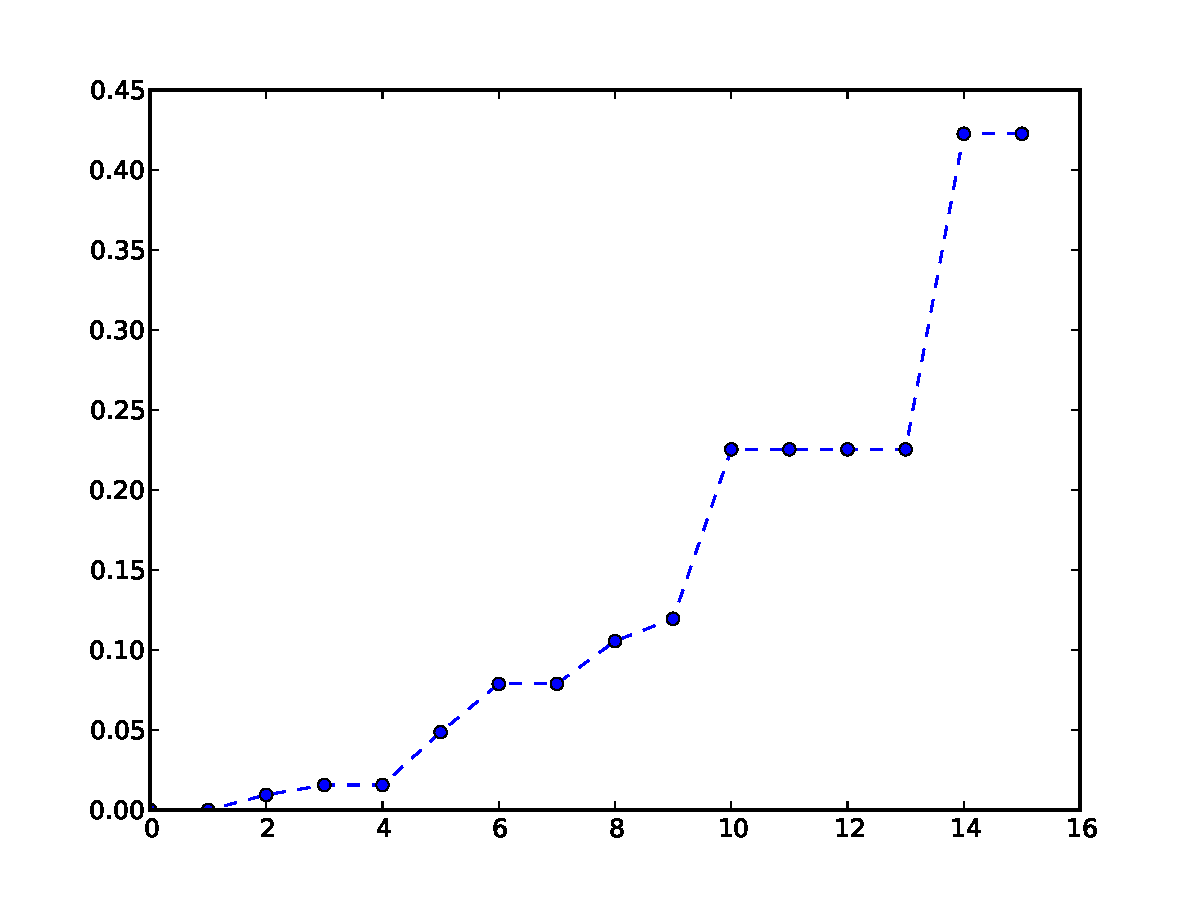
\includegraphics{index-1.pdf}

Returns hierarchically clustered object

Parameters:

Returns:

Examples

Notes
\begin{quote}

This hclust function is not quite right for the MI case. Need a generic MI function that can take in clusters of RV's, not just single ones 
Use the ``grouping property'' as discussed by Kraskov paper.
\end{quote}

\end{fulllineitems}

\index{normal() (in module halla.hierarchy)}

\begin{fulllineitems}
\phantomsection\label{index:halla.hierarchy.normal}\pysiglinewithargsret{\code{halla.hierarchy.}\bfcode{normal}}{\emph{loc=0.0}, \emph{scale=1.0}, \emph{size=None}}{}
Draw random samples from a normal (Gaussian) distribution.

The probability density function of the normal distribution, first
derived by De Moivre and 200 years later by both Gauss and Laplace
independently {\color{red}\bfseries{}{[}2{]}\_}, is often called the bell curve because of
its characteristic shape (see the example below).

The normal distributions occurs often in nature.  For example, it
describes the commonly occurring distribution of samples influenced
by a large number of tiny, random disturbances, each with its own
unique distribution {\color{red}\bfseries{}{[}2{]}\_}.
\begin{description}
\item[{loc}] \leavevmode{[}float{]}
Mean (``centre'') of the distribution.

\item[{scale}] \leavevmode{[}float{]}
Standard deviation (spread or ``width'') of the distribution.

\item[{size}] \leavevmode{[}tuple of ints{]}
Output shape.  If the given shape is, e.g., \code{(m, n, k)}, then
\code{m * n * k} samples are drawn.

\end{description}
\begin{description}
\item[{scipy.stats.distributions.norm}] \leavevmode{[}probability density function,{]}
distribution or cumulative density function, etc.

\end{description}

The probability density for the Gaussian distribution is
\begin{equation}p(x) = \frac{1}{\sqrt{ 2 \pi \sigma^2 }}e^{ - \frac{ (x - \mu)^2 } {2 \sigma^2} },\end{equation}
where $\mu$ is the mean and $\sigma$ the standard deviation.
The square of the standard deviation, $\sigma^2$, is called the
variance.

The function has its peak at the mean, and its ``spread'' increases with
the standard deviation (the function reaches 0.607 times its maximum at
$x + \sigma$ and $x - \sigma$ {\color{red}\bfseries{}{[}2{]}\_}).  This implies that
\emph{numpy.random.normal} is more likely to return samples lying close to the
mean, rather than those far away.

Draw samples from the distribution:

\begin{Verbatim}[commandchars=\\\{\}]
\PYG{g+gp}{\PYGZgt{}\PYGZgt{}\PYGZgt{} }\PYG{n}{mu}\PYG{p}{,} \PYG{n}{sigma} \PYG{o}{=} \PYG{l+m+mi}{0}\PYG{p}{,} \PYG{l+m+mf}{0.1} \PYG{c}{\PYGZsh{} mean and standard deviation}
\PYG{g+gp}{\PYGZgt{}\PYGZgt{}\PYGZgt{} }\PYG{n}{s} \PYG{o}{=} \PYG{n}{np}\PYG{o}{.}\PYG{n}{random}\PYG{o}{.}\PYG{n}{normal}\PYG{p}{(}\PYG{n}{mu}\PYG{p}{,} \PYG{n}{sigma}\PYG{p}{,} \PYG{l+m+mi}{1000}\PYG{p}{)}
\end{Verbatim}

Verify the mean and the variance:

\begin{Verbatim}[commandchars=\\\{\}]
\PYG{g+gp}{\PYGZgt{}\PYGZgt{}\PYGZgt{} }\PYG{n+nb}{abs}\PYG{p}{(}\PYG{n}{mu} \PYG{o}{\PYGZhy{}} \PYG{n}{np}\PYG{o}{.}\PYG{n}{mean}\PYG{p}{(}\PYG{n}{s}\PYG{p}{)}\PYG{p}{)} \PYG{o}{\PYGZlt{}} \PYG{l+m+mf}{0.01}
\PYG{g+go}{True}
\end{Verbatim}

\begin{Verbatim}[commandchars=\\\{\}]
\PYG{g+gp}{\PYGZgt{}\PYGZgt{}\PYGZgt{} }\PYG{n+nb}{abs}\PYG{p}{(}\PYG{n}{sigma} \PYG{o}{\PYGZhy{}} \PYG{n}{np}\PYG{o}{.}\PYG{n}{std}\PYG{p}{(}\PYG{n}{s}\PYG{p}{,} \PYG{n}{ddof}\PYG{o}{=}\PYG{l+m+mi}{1}\PYG{p}{)}\PYG{p}{)} \PYG{o}{\PYGZlt{}} \PYG{l+m+mf}{0.01}
\PYG{g+go}{True}
\end{Verbatim}

Display the histogram of the samples, along with
the probability density function:

\begin{Verbatim}[commandchars=\\\{\}]
\PYG{g+gp}{\PYGZgt{}\PYGZgt{}\PYGZgt{} }\PYG{k+kn}{import} \PYG{n+nn}{matplotlib.pyplot} \PYG{k+kn}{as} \PYG{n+nn}{plt}
\PYG{g+gp}{\PYGZgt{}\PYGZgt{}\PYGZgt{} }\PYG{n}{count}\PYG{p}{,} \PYG{n}{bins}\PYG{p}{,} \PYG{n}{ignored} \PYG{o}{=} \PYG{n}{plt}\PYG{o}{.}\PYG{n}{hist}\PYG{p}{(}\PYG{n}{s}\PYG{p}{,} \PYG{l+m+mi}{30}\PYG{p}{,} \PYG{n}{normed}\PYG{o}{=}\PYG{n+nb+bp}{True}\PYG{p}{)}
\PYG{g+gp}{\PYGZgt{}\PYGZgt{}\PYGZgt{} }\PYG{n}{plt}\PYG{o}{.}\PYG{n}{plot}\PYG{p}{(}\PYG{n}{bins}\PYG{p}{,} \PYG{l+m+mi}{1}\PYG{o}{/}\PYG{p}{(}\PYG{n}{sigma} \PYG{o}{*} \PYG{n}{np}\PYG{o}{.}\PYG{n}{sqrt}\PYG{p}{(}\PYG{l+m+mi}{2} \PYG{o}{*} \PYG{n}{np}\PYG{o}{.}\PYG{n}{pi}\PYG{p}{)}\PYG{p}{)} \PYG{o}{*}
\PYG{g+gp}{... }               \PYG{n}{np}\PYG{o}{.}\PYG{n}{exp}\PYG{p}{(} \PYG{o}{\PYGZhy{}} \PYG{p}{(}\PYG{n}{bins} \PYG{o}{\PYGZhy{}} \PYG{n}{mu}\PYG{p}{)}\PYG{o}{*}\PYG{o}{*}\PYG{l+m+mi}{2} \PYG{o}{/} \PYG{p}{(}\PYG{l+m+mi}{2} \PYG{o}{*} \PYG{n}{sigma}\PYG{o}{*}\PYG{o}{*}\PYG{l+m+mi}{2}\PYG{p}{)} \PYG{p}{)}\PYG{p}{,}
\PYG{g+gp}{... }         \PYG{n}{linewidth}\PYG{o}{=}\PYG{l+m+mi}{2}\PYG{p}{,} \PYG{n}{color}\PYG{o}{=}\PYG{l+s}{\PYGZsq{}}\PYG{l+s}{r}\PYG{l+s}{\PYGZsq{}}\PYG{p}{)}
\PYG{g+gp}{\PYGZgt{}\PYGZgt{}\PYGZgt{} }\PYG{n}{plt}\PYG{o}{.}\PYG{n}{show}\PYG{p}{(}\PYG{p}{)}
\end{Verbatim}

\end{fulllineitems}

\index{one\_against\_one() (in module halla.hierarchy)}

\begin{fulllineitems}
\phantomsection\label{index:halla.hierarchy.one_against_one}\pysiglinewithargsret{\code{halla.hierarchy.}\bfcode{one\_against\_one}}{\emph{pClusterNode1}, \emph{pClusterNode2}, \emph{pArray1}, \emph{pArray2}}{}
one\_against\_one hypothesis testing for a particular layer

Input: pClusterNode1, pClusterNode2, pArray1, pArray2

Output: aiIndex1, aiIndex2, pVal

\end{fulllineitems}

\index{recursive\_all\_against\_all() (in module halla.hierarchy)}

\begin{fulllineitems}
\phantomsection\label{index:halla.hierarchy.recursive_all_against_all}\pysiglinewithargsret{\code{halla.hierarchy.}\bfcode{recursive\_all\_against\_all}}{\emph{apClusterNode1}, \emph{apClusterNode2}, \emph{pArray1}, \emph{pArray2}, \emph{pOut=}\optional{}, \emph{pFDR=\textless{}function bh at 0x6f80938\textgreater{}}}{}
Performs recursive all-against-all (the default HAllA routine) with fdr correction

Input: apClusterNode1, apClusterNode2, pArray1, pArray2, pFDR

Output: a list of ( (aiIndex1, pBag1), (aiIndex2, pBag2) )

\end{fulllineitems}

\index{reduce\_tree() (in module halla.hierarchy)}

\begin{fulllineitems}
\phantomsection\label{index:halla.hierarchy.reduce_tree}\pysiglinewithargsret{\code{halla.hierarchy.}\bfcode{reduce\_tree}}{\emph{pClusterNode}, \emph{pFunction=\textless{}function \textless{}lambda\textgreater{} at 0x7840cf8\textgreater{}}, \emph{aOut=}\optional{}}{}
Recursive

Input: pClusterNode, pFunction = lambda x: x.id, aOut = {[}{]}

Output: a list of pFunction calls (node ids by default)

\end{fulllineitems}

\index{reduce\_tree\_by\_layer() (in module halla.hierarchy)}

\begin{fulllineitems}
\phantomsection\label{index:halla.hierarchy.reduce_tree_by_layer}\pysiglinewithargsret{\code{halla.hierarchy.}\bfcode{reduce\_tree\_by\_layer}}{\emph{apParents}, \emph{iLevel=0}, \emph{iStop=None}}{}
Traverse one tree.

Input: apParents, iLevel = 0, iStop = None

Output: a list of (iLevel, list\_of\_nodes\_at\_iLevel)

\end{fulllineitems}

\index{traverse\_by\_layer() (in module halla.hierarchy)}

\begin{fulllineitems}
\phantomsection\label{index:halla.hierarchy.traverse_by_layer}\pysiglinewithargsret{\code{halla.hierarchy.}\bfcode{traverse\_by\_layer}}{\emph{pClusterNode1}, \emph{pClusterNode2}, \emph{pArray1}, \emph{pArray2}, \emph{pFunction}}{}~\begin{quote}

Useful function for doing all-against-all comparison between nodes in each layer

traverse two trees at once, applying function \emph{pFunction} to each layer pair

latex: \$pFunction: data1        imes data2
\end{quote}

ightarrow mathbb\{R\}\textasciicircum{}k, \$ for \$k\$ the size of the cross-product set per layer
\begin{quote}

Input: pClusterNode1, pClusterNode2, pArray1, pArray2, pFunction
Output: (i,j), pFunction( pArray{[}:,i{]}, pArray2{[}:,j{]})
\end{quote}

\end{fulllineitems}

\index{truncate\_tree() (in module halla.hierarchy)}

\begin{fulllineitems}
\phantomsection\label{index:halla.hierarchy.truncate_tree}\pysiglinewithargsret{\code{halla.hierarchy.}\bfcode{truncate\_tree}}{\emph{apClusterNode}, \emph{iSkip}, \emph{iLevel=0}}{}
Chop tree from root, returning smaller tree towards the leaves

Input: pClusterNode, iLevel

Output: list of ClusterNodes

\end{fulllineitems}



\section{Indices and tables}
\label{index:indices-and-tables}\begin{itemize}
\item {} 
\emph{genindex}

\item {} 
\emph{modindex}

\item {} 
\emph{search}

\end{itemize}


\section{License}
\label{index:license}
This software is licensed under the MIT license.

Copyright (c) 2013 Yo Sup Moon, Curtis Huttenhower

Permission is hereby granted, free of charge, to any person obtaining a copy of this software and associated documentation files (the ``Software''), to deal in the Software without restriction, including without limitation the rights to use, copy, modify, merge, publish, distribute, sublicense, and/or sell copies of the Software, and to permit persons to whom the Software is furnished to do so, subject to the following conditions:

The above copyright notice and this permission notice shall be included in all copies or substantial portions of the Software.

THE SOFTWARE IS PROVIDED ``AS IS'', WITHOUT WARRANTY OF ANY KIND, EXPRESS OR IMPLIED, INCLUDING BUT NOT LIMITED TO THE WARRANTIES OF MERCHANTABILITY, FITNESS FOR A PARTICULAR PURPOSE AND NONINFRINGEMENT. IN NO EVENT SHALL THE AUTHORS OR COPYRIGHT HOLDERS BE LIABLE FOR ANY CLAIM, DAMAGES OR OTHER LIABILITY, WHETHER IN AN ACTION OF CONTRACT, TORT OR OTHERWISE, ARISING FROM, OUT OF OR IN CONNECTION WITH THE SOFTWARE OR THE USE OR OTHER DEALINGS IN THE SOFTWARE.


\renewcommand{\indexname}{Python Module Index}
\begin{theindex}
\def\bigletter#1{{\Large\sffamily#1}\nopagebreak\vspace{1mm}}
\bigletter{h}
\item {\texttt{halla.distance}}, \pageref{index:module-halla.distance}
\item {\texttt{halla.hierarchy}}, \pageref{index:module-halla.hierarchy}
\item {\texttt{halla.logger}}, \pageref{index:module-halla.logger}
\item {\texttt{halla.parser}}, \pageref{index:module-halla.parser}
\item {\texttt{halla.stats}}, \pageref{index:module-halla.stats}
\item {\texttt{halla.test}}, \pageref{index:module-halla.test}
\end{theindex}

\renewcommand{\indexname}{Index}
\printindex
\end{document}
